\section{Method}\label{sec:method}
% Spatial correlation 2d histograms (den nemme, 1 2d hist)
In this section, we will describe the method for exploiting spatial correlation based on the
2D-histograms of the tomographies. We will start by motivating the problem, then give an overview
of how we solve the problem, with a final detailed walkthrough of each step in the overall workflow.

\subsection{1-dimensional histograms}
%diskuter overlappende materialer
Looking at a 1D-histogram of the voxel value in a tomography, as shown in~\Cref{fig:1d-hist}, we are
able to distinguish different distributions, but we see that there are large overlaps. This leads to
global thresholding being infeasible, at least for the distributions in the lower half of the histogram.
This happens because the voxel value is not globally defined, as~\Cref{sec:physics} explains, which
illustrates how the different materials cover ranges of values that blend together in the histogram.

\begin{figure}
    \centering
    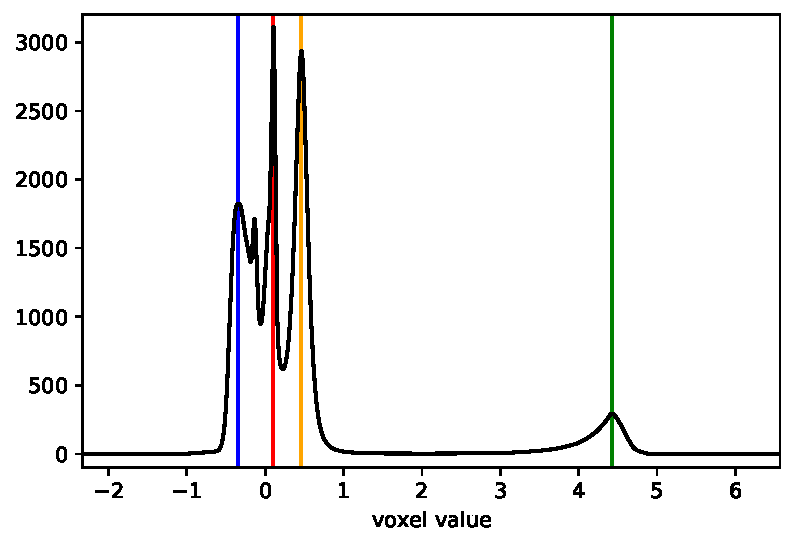
\includegraphics[width=\linewidth]{1d_hist.pdf}
    \caption{1-dimensional histogram of the voxel values of a tomography. The blue line is air peak,
    the red line is the soft tissue peak, the green line is the bone peak, and the orange line is
    the implant peak.}
    \label{fig:1d-hist}
\end{figure}

\subsection{Preprocessing}\label{sec:preprocess}
To reduce the complexity of the segmentation process, we preprocess
the data by removing redundant information.
% Since the values of the implant material is well-separated from the rest of the sample, obtaining
% the rough implant mask through global thresholding is trivial, as the orange line in~\Cref{fig:1d-hist}
% shows. This mask is then refined, along with the internal gaps being closed, giving us the implant mask.
We first compute a coarse
bone-region using a crude segmentation, and through a direct geometric
analysis of the implant determines the sample coordinate system, with the origin
on the back-plane of the sawed-through implants and principal axes coordinate system vectors
$\mathbf{u}$ pointing up towards the implant top, $\mathbf{v}$ pointing forward away from the back-plane,
and $\mathbf{w}$ point right, parallel to the back-plane. An automatic wave-analysis of the threads
computationally determines the macro-threaded recipient bone region, and the micro-threaded de-novo regenerated bone region.
We then perform the spatially-aware segmentation analysis restricted to the bone-regions in order to
not expand effort on the parts of the segmentation problem that can be solved with simpler methods.
Note that the process is fully automatic, and does not require human intervention.

%TODO: Måske medtage disse detaljer, men er for træt til at renskrive.
% , we are also able to remove the air making up half of the sample cylinder. This is depicted
% in~\Cref{fig:3viewsample}, above the implant and to the left of the implant in the XY and YZ cross
% sections respectively. Finally the implant mask can show us the orientation of the implant. This squashes
% the blue peak from the histogram, leaving the two peaks marked by the red and green lines as being
% the most defined.

% As we are only interested in the voxels inside the bone, and we know that bone is the most prominent
% material left, we perform another coarse segmentation. This is done by thresholding between the two
% large distributions, choosing everything to the right of this threshold as the bone mask. These voxels
% are morphologically closed, to also consumes the internal gaps in the bone region, which makes up the
% soft tissue inside the bone. The implant and bone region masks are applied throughout subsequent steps
% to filter out noise in the tomography.

\subsection{Exploiting spatial information}
% Show the correlation of x,y,z,r to histograms 2d
Our goal is to discover how the value distributions for the different materials -- bone, blood vessels, etc. --
change as a function of space. In other words, we wish to uncover information about the conditional probabilities $P(m|v,\xx)$ that a voxel with value $v$ and
position $\xx$ represents material $m$. We cannot compute this directly using only the image, as only one voxel occupies position $\xx$. 

However, if we fix one axis $x$, $y$, or $z$, the image {\em does} contain millions of voxels with that fixed value, enough to make good statistical
models for e.g.~the conditional probabilities $P(m|v,x)$, $P(m|v,y)$, and $P(m|v,z)$. To this end, we compute 2D histograms that simply count voxel frequencies
both conditioned on value $v$ and coordinate value along either $x$, $y$, or $z$. 

Figure \ref{fig:2dhists}(a)
shows the histogram for our model tomogram (implant excluded) as a function of the $y$ coordinate: each row in the image is a histogram for a fixed value of $y$.
Figure \ref{fig:3viewsample}(a) helps us see what happens: For $y<2400\micron$, there is only air, then we reach a thin layer of resin, after which we enter
the region where we find bone, soft tissue, resin, and air. The air voxels are brightened as we approach the implant, shifting the peaks smoothly rightwards.
Figure \ref{fig:2dhists}(b) shows a similar 2D histogram for the radial coordinate $r=\sqrt{x^2+y^2+z^2}$.
From this plot, we see two prominent distributions that change along the $r$ axis. The radius correlates with distance to the sample surface
(capturing edge effects), and for medium $r$, it is a good proxy for distance to the implant, and we see a brightening with smaller $r$, and a darkening and
broadening of the distributions for large $r$. Each {\em view} provides us with additional information about how voxel values are distorted throughout space:
analogous to casting shadows along different axes to obtain more information about a 3D object. We can either use Bayesian statistics to combine information
from multiple axes, or construct a spatial grouping that is particularly suited to capture the effects of the distortive effects that we want to counter.
The next section describes the latter.

% Kept for historical reasons.
%\begin{algorithm}
%    \caption{2-dimensional histograms. Allocation also implies zero initialization.}
%    \label{alg:2dhists}
%    \begin{algorithmic}
%        \Function {2D\_hist} {$voxels[n_z,n_y,n_x],c_x,c_y,n_{bins},v_{min},v_{max}$}
%            \State $n_r \gets \left\lfloor\sqrt{\left\lfloor \frac{n_x}{2} \right\rfloor^2 + \left\lfloor \frac{n_y}{2} \right\rfloor^2}\right\rfloor+1$
%            \State \textbf{allocate} $h_z[n_z,n_{bins}], h_y[n_y,n_{bins}]$
%            \State \textbf{allocate} $h_x[n_x,n_{bins}], h_r[n_r,n_{bins}]$
%            \For {$z,y,x$ \textbf{in} $0{:}n_z,0{:}n_y,0{:}n_x$}
%                \State $v \gets voxels[z,y,x]$
%                \If {$v_{min} \leq v \leq v_{max}$}
%                    \State $v_{i} \gets (n_{bins}-1) \cdot \frac{v - v_{min}}{v_{max} - v_{min}}$
%                    \State $r \gets \left\lfloor\sqrt{(x-c_x)^2 + (y-c_y)^2}\right\rfloor$
%                    \State $h_z[z,v_{i}]{+}{+}$
%                    \State $h_y[y,v_{i}]{+}{+}$
%                    \State $h_x[x,v_{i}]{+}{+}$
%                    \State $h_r[r,v_{i}]{+}{+}$
%                \EndIf
%            \EndFor
%            \Return $h_z,h_y,h_z,h_r$
%        \EndFunction
%    \end{algorithmic}
%\end{algorithm}

\begin{algorithm}
    \caption{2-dimensional radius histogram.}
    \label{alg:2dhists}
    \begin{algorithmic}
        \Function {hist\_r} {$voxels[n_z,n_y,n_x],c_x,c_y,n_{bins},v_{min},v_{max}$}
            \For {$z,y,x$ \textbf{in} $0{:}n_z,0{:}n_y,0{:}n_x$}
                \State $v \gets voxels[z,y,x]$
                \If {$v_{min} \leq v \leq v_{max}$}
                    \State $v_{i} \gets (n_{bins}-1) \cdot \frac{v - v_{min}}{v_{max} - v_{min}}$
                    \State $r \gets \left\lfloor\sqrt{(x-c_x)^2 + (y-c_y)^2}\right\rfloor$
                    \State $h_r[r,v_{i}]{+}{+}$
                \EndIf
            \EndFor
            \Return $h_r$
        \EndFunction
    \end{algorithmic}
\end{algorithm}

\begin{figure}
    \centering
    %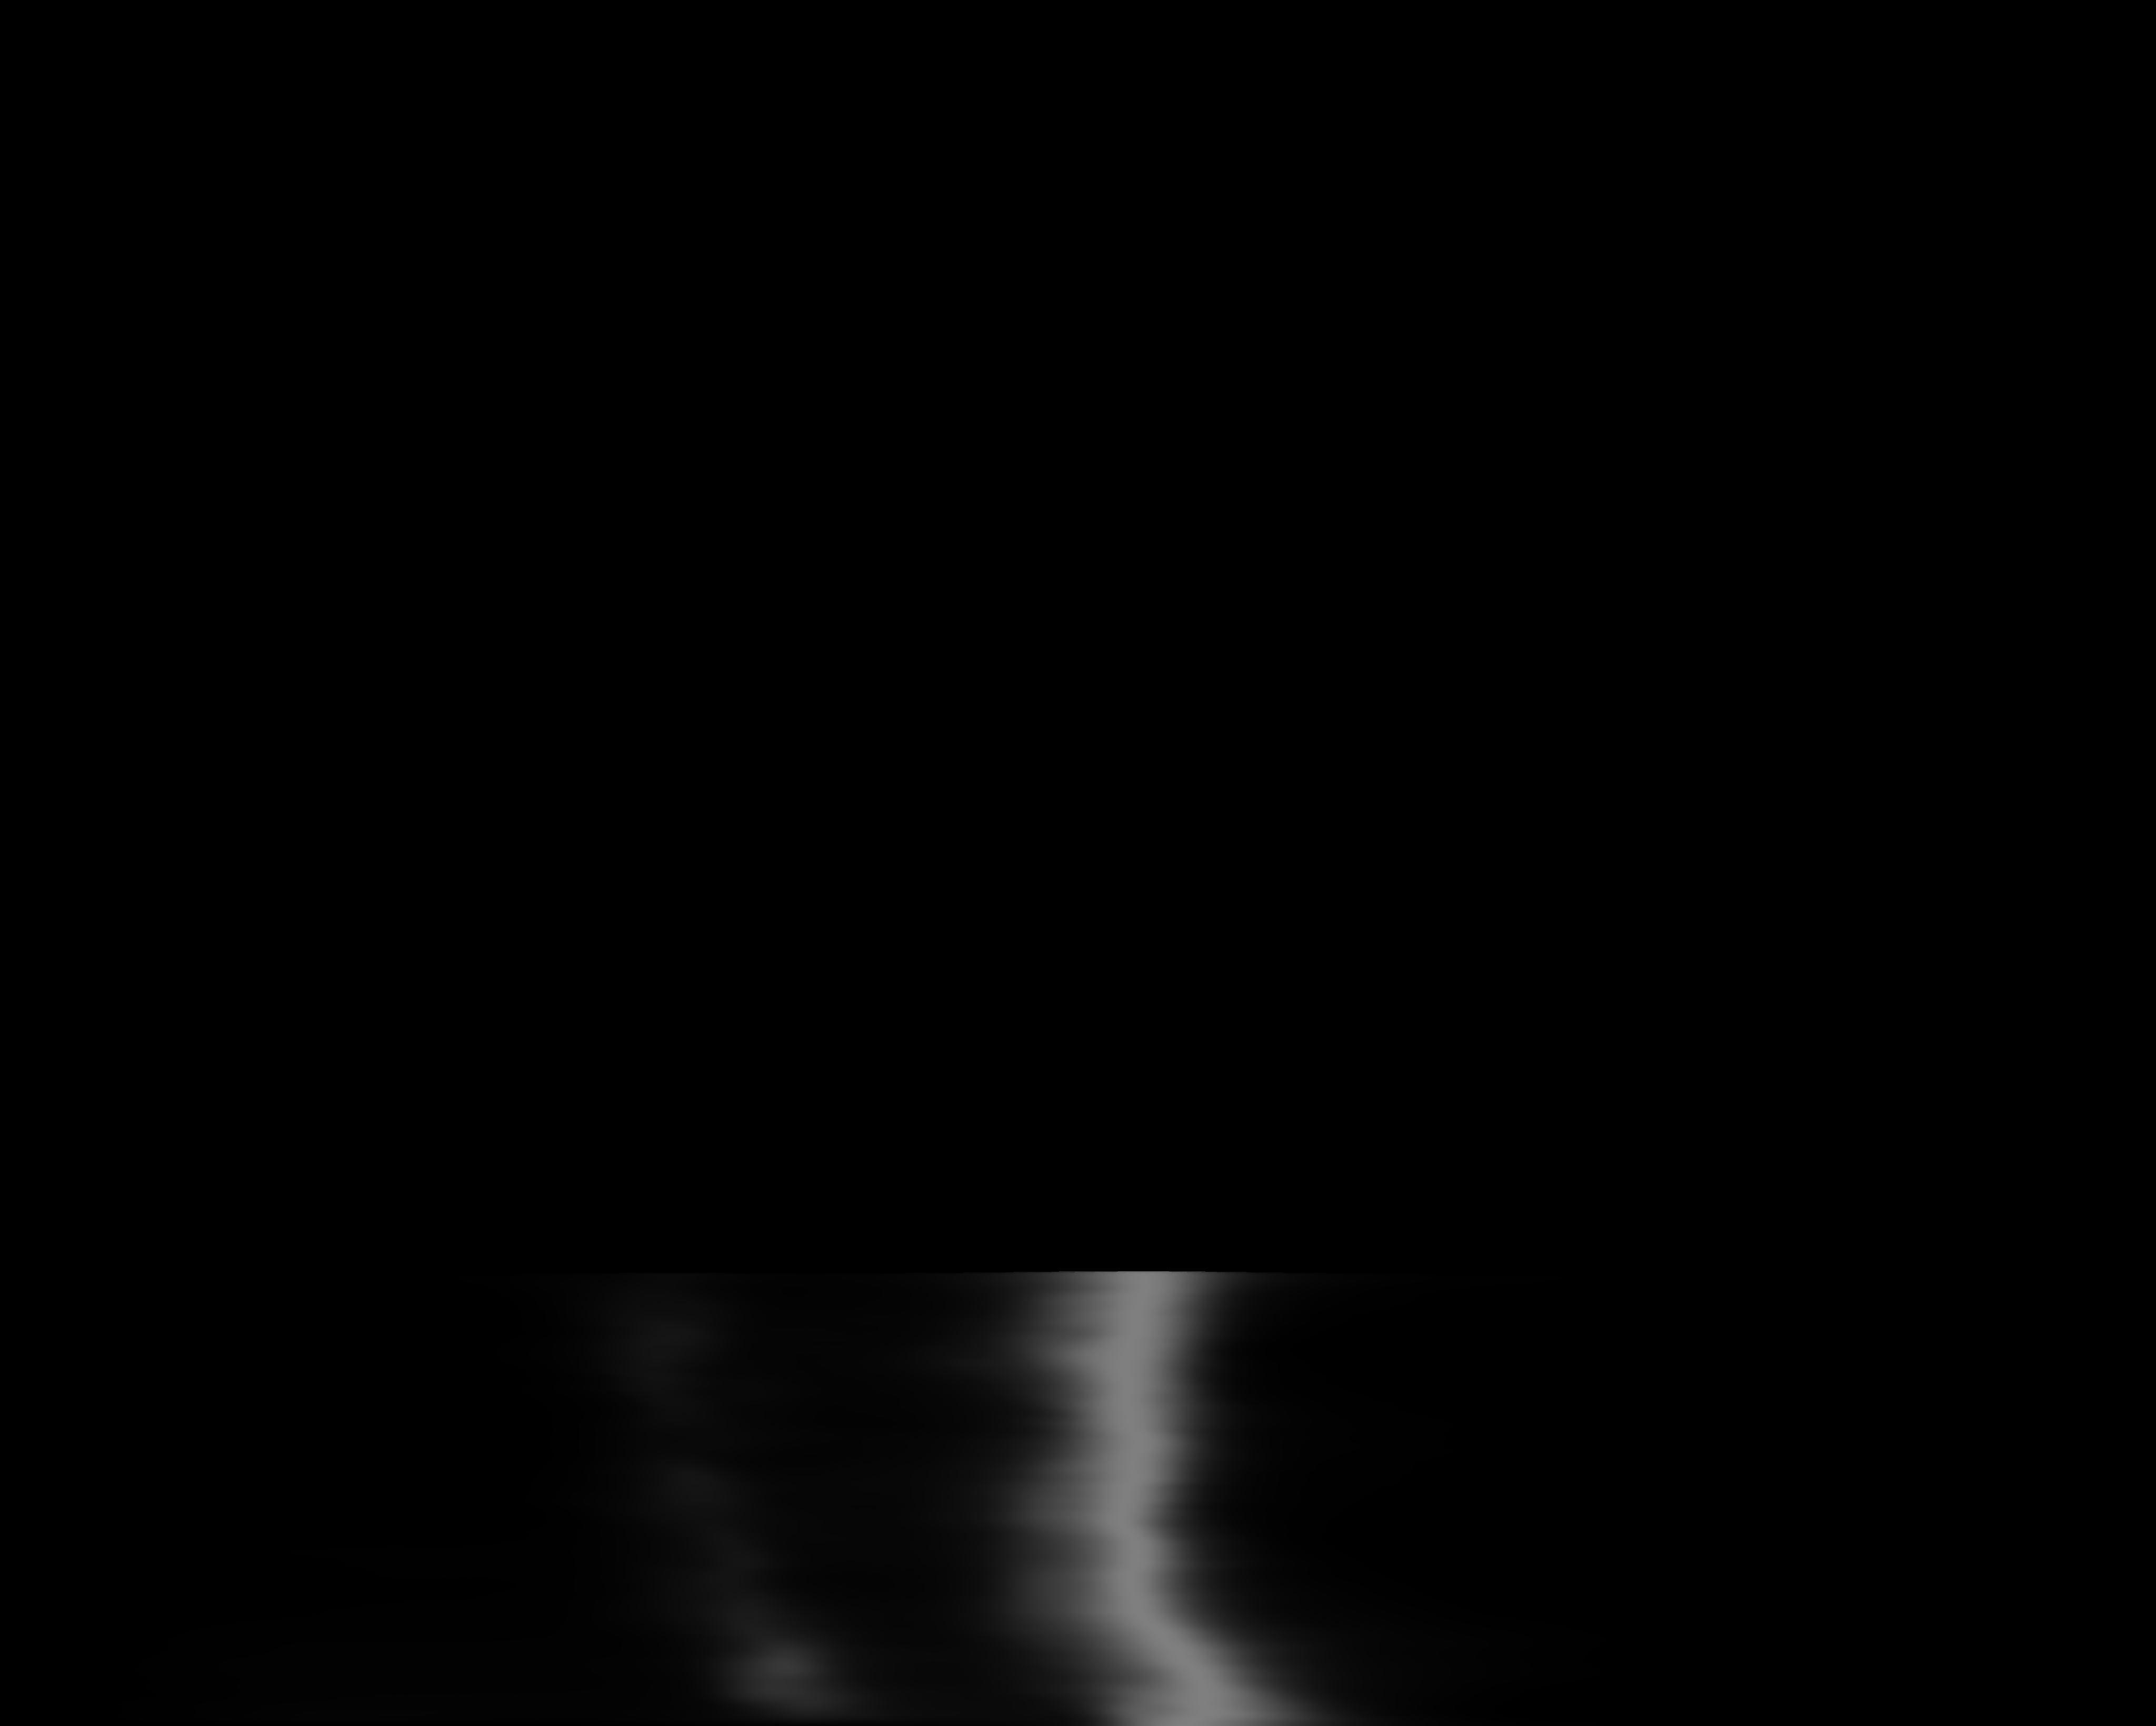
\includegraphics[width=.49\linewidth]{zb-bone_region3.png}
    %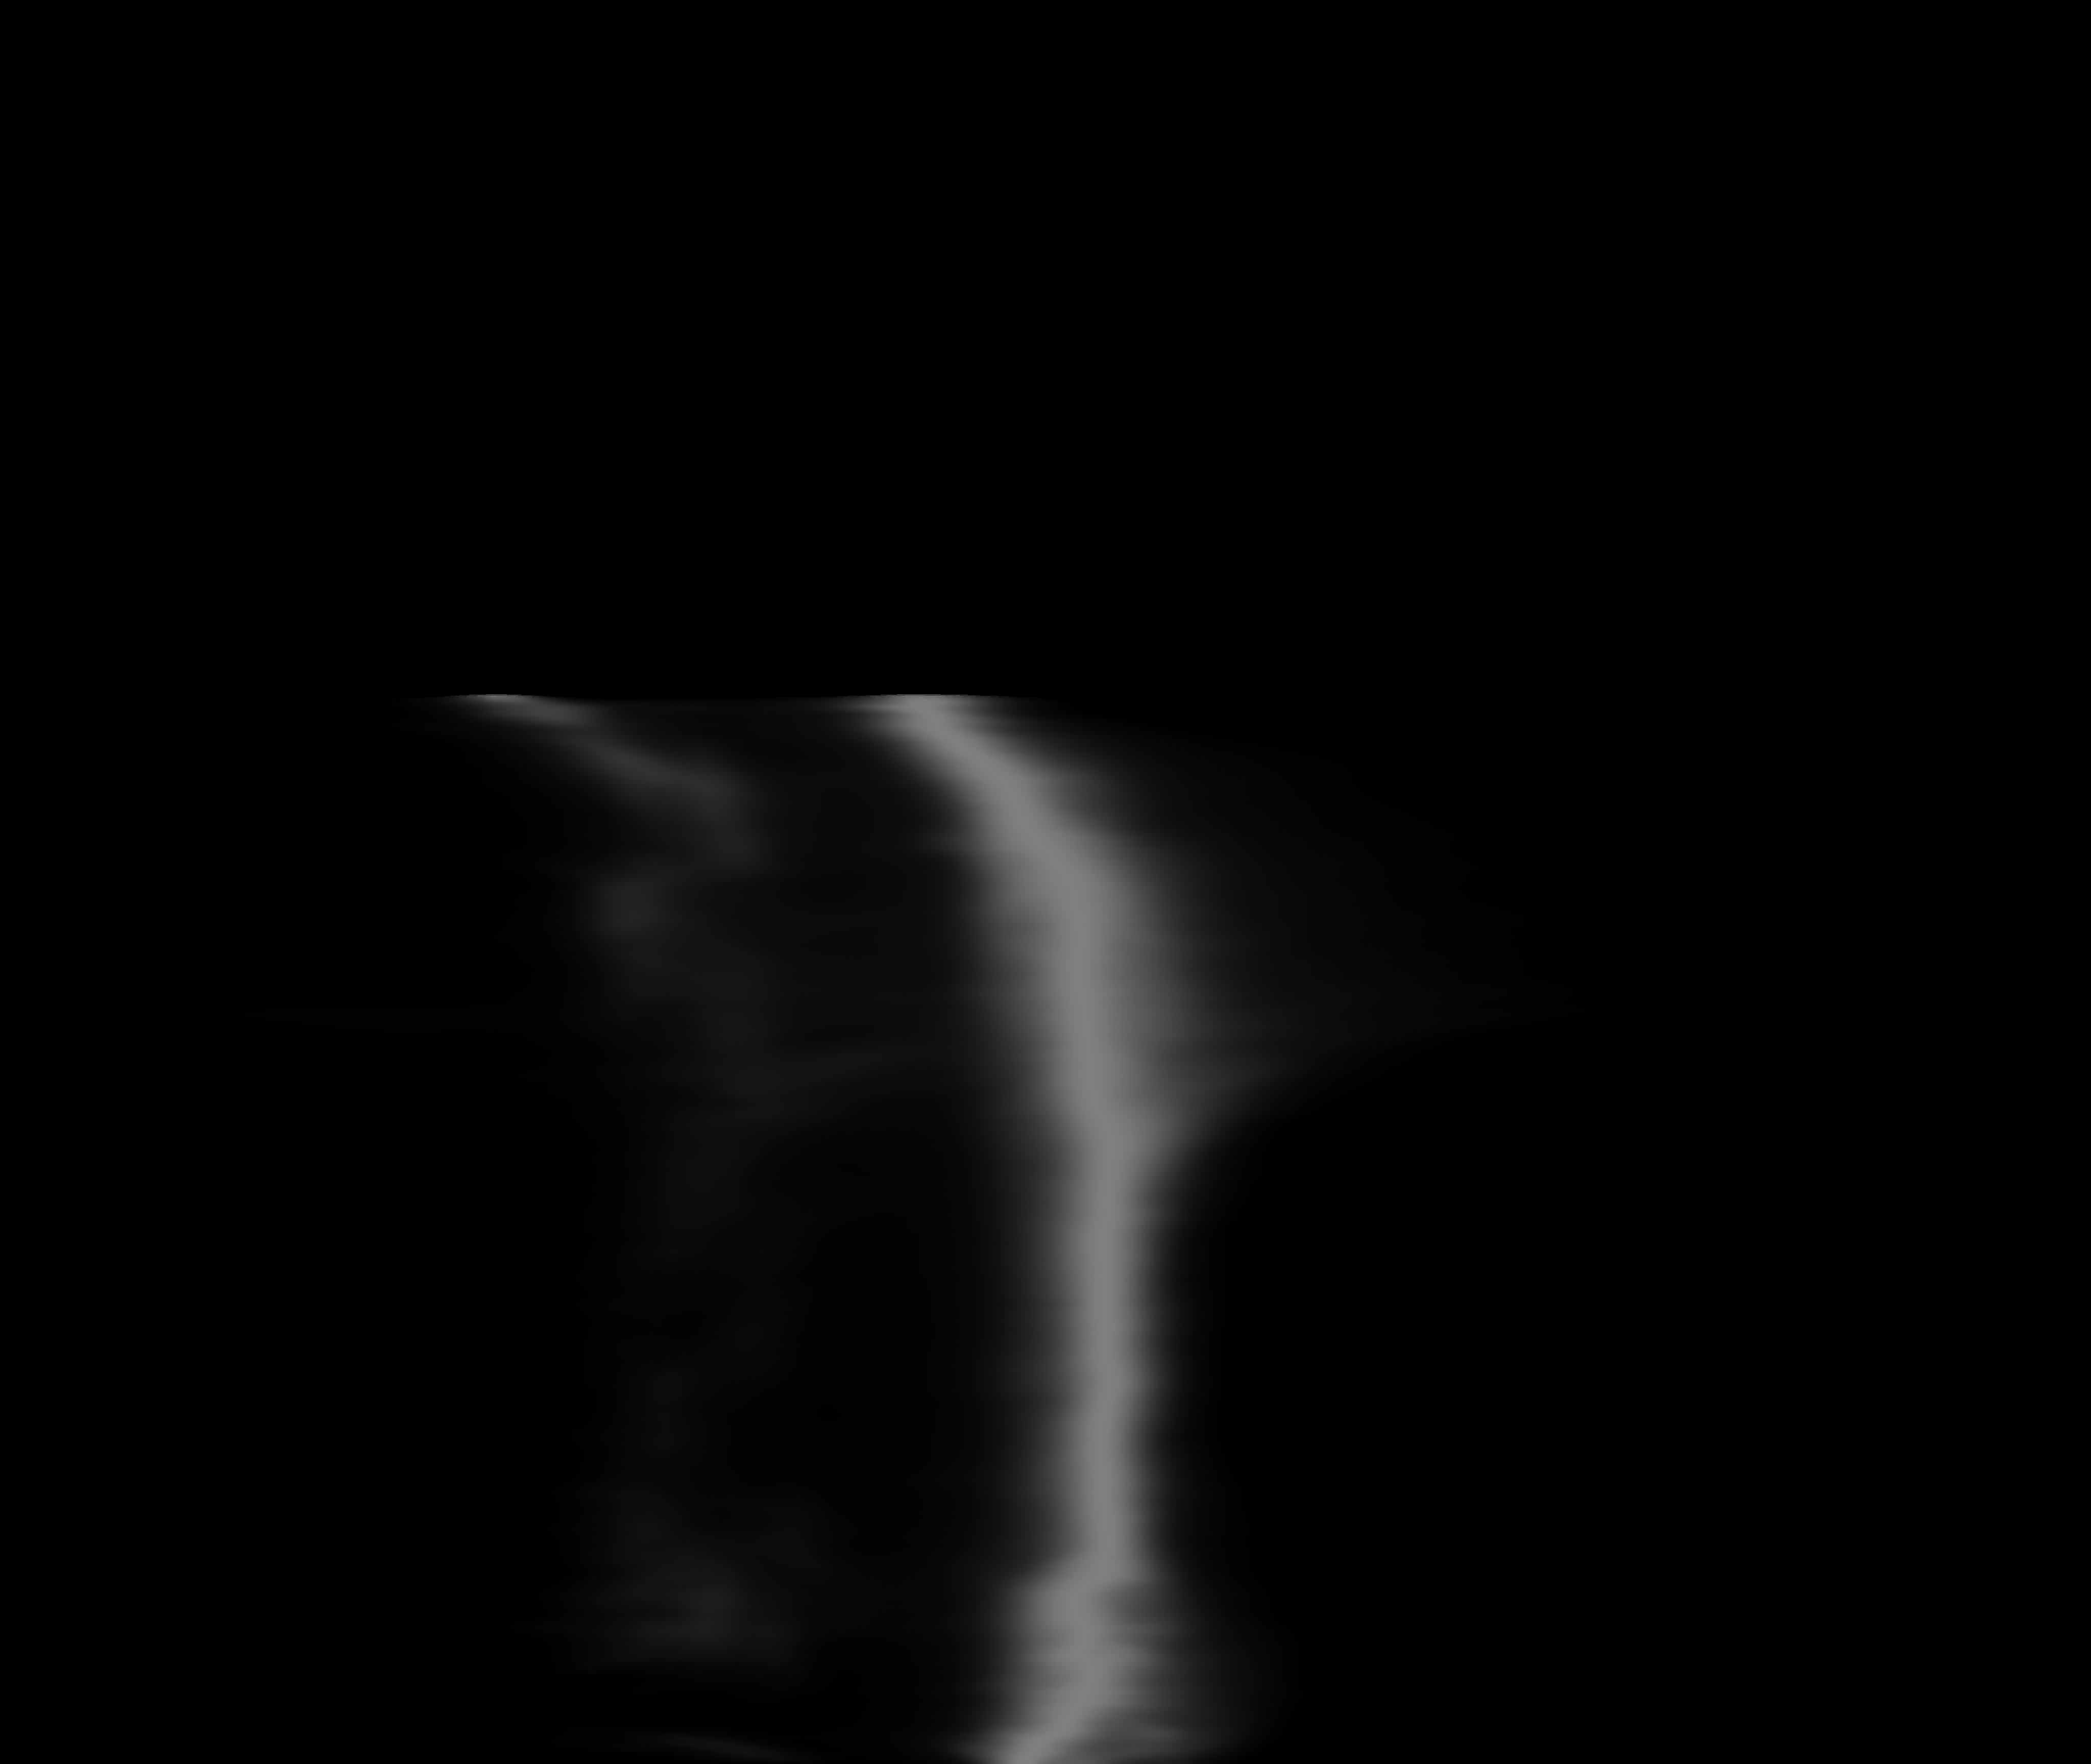
\includegraphics[width=.49\linewidth]{yb-bone_region3.png}
    %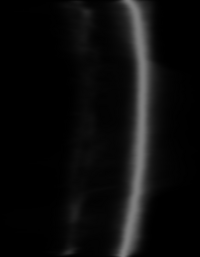
\includegraphics[width=.49\linewidth]{xb-bone_region3.png}
    %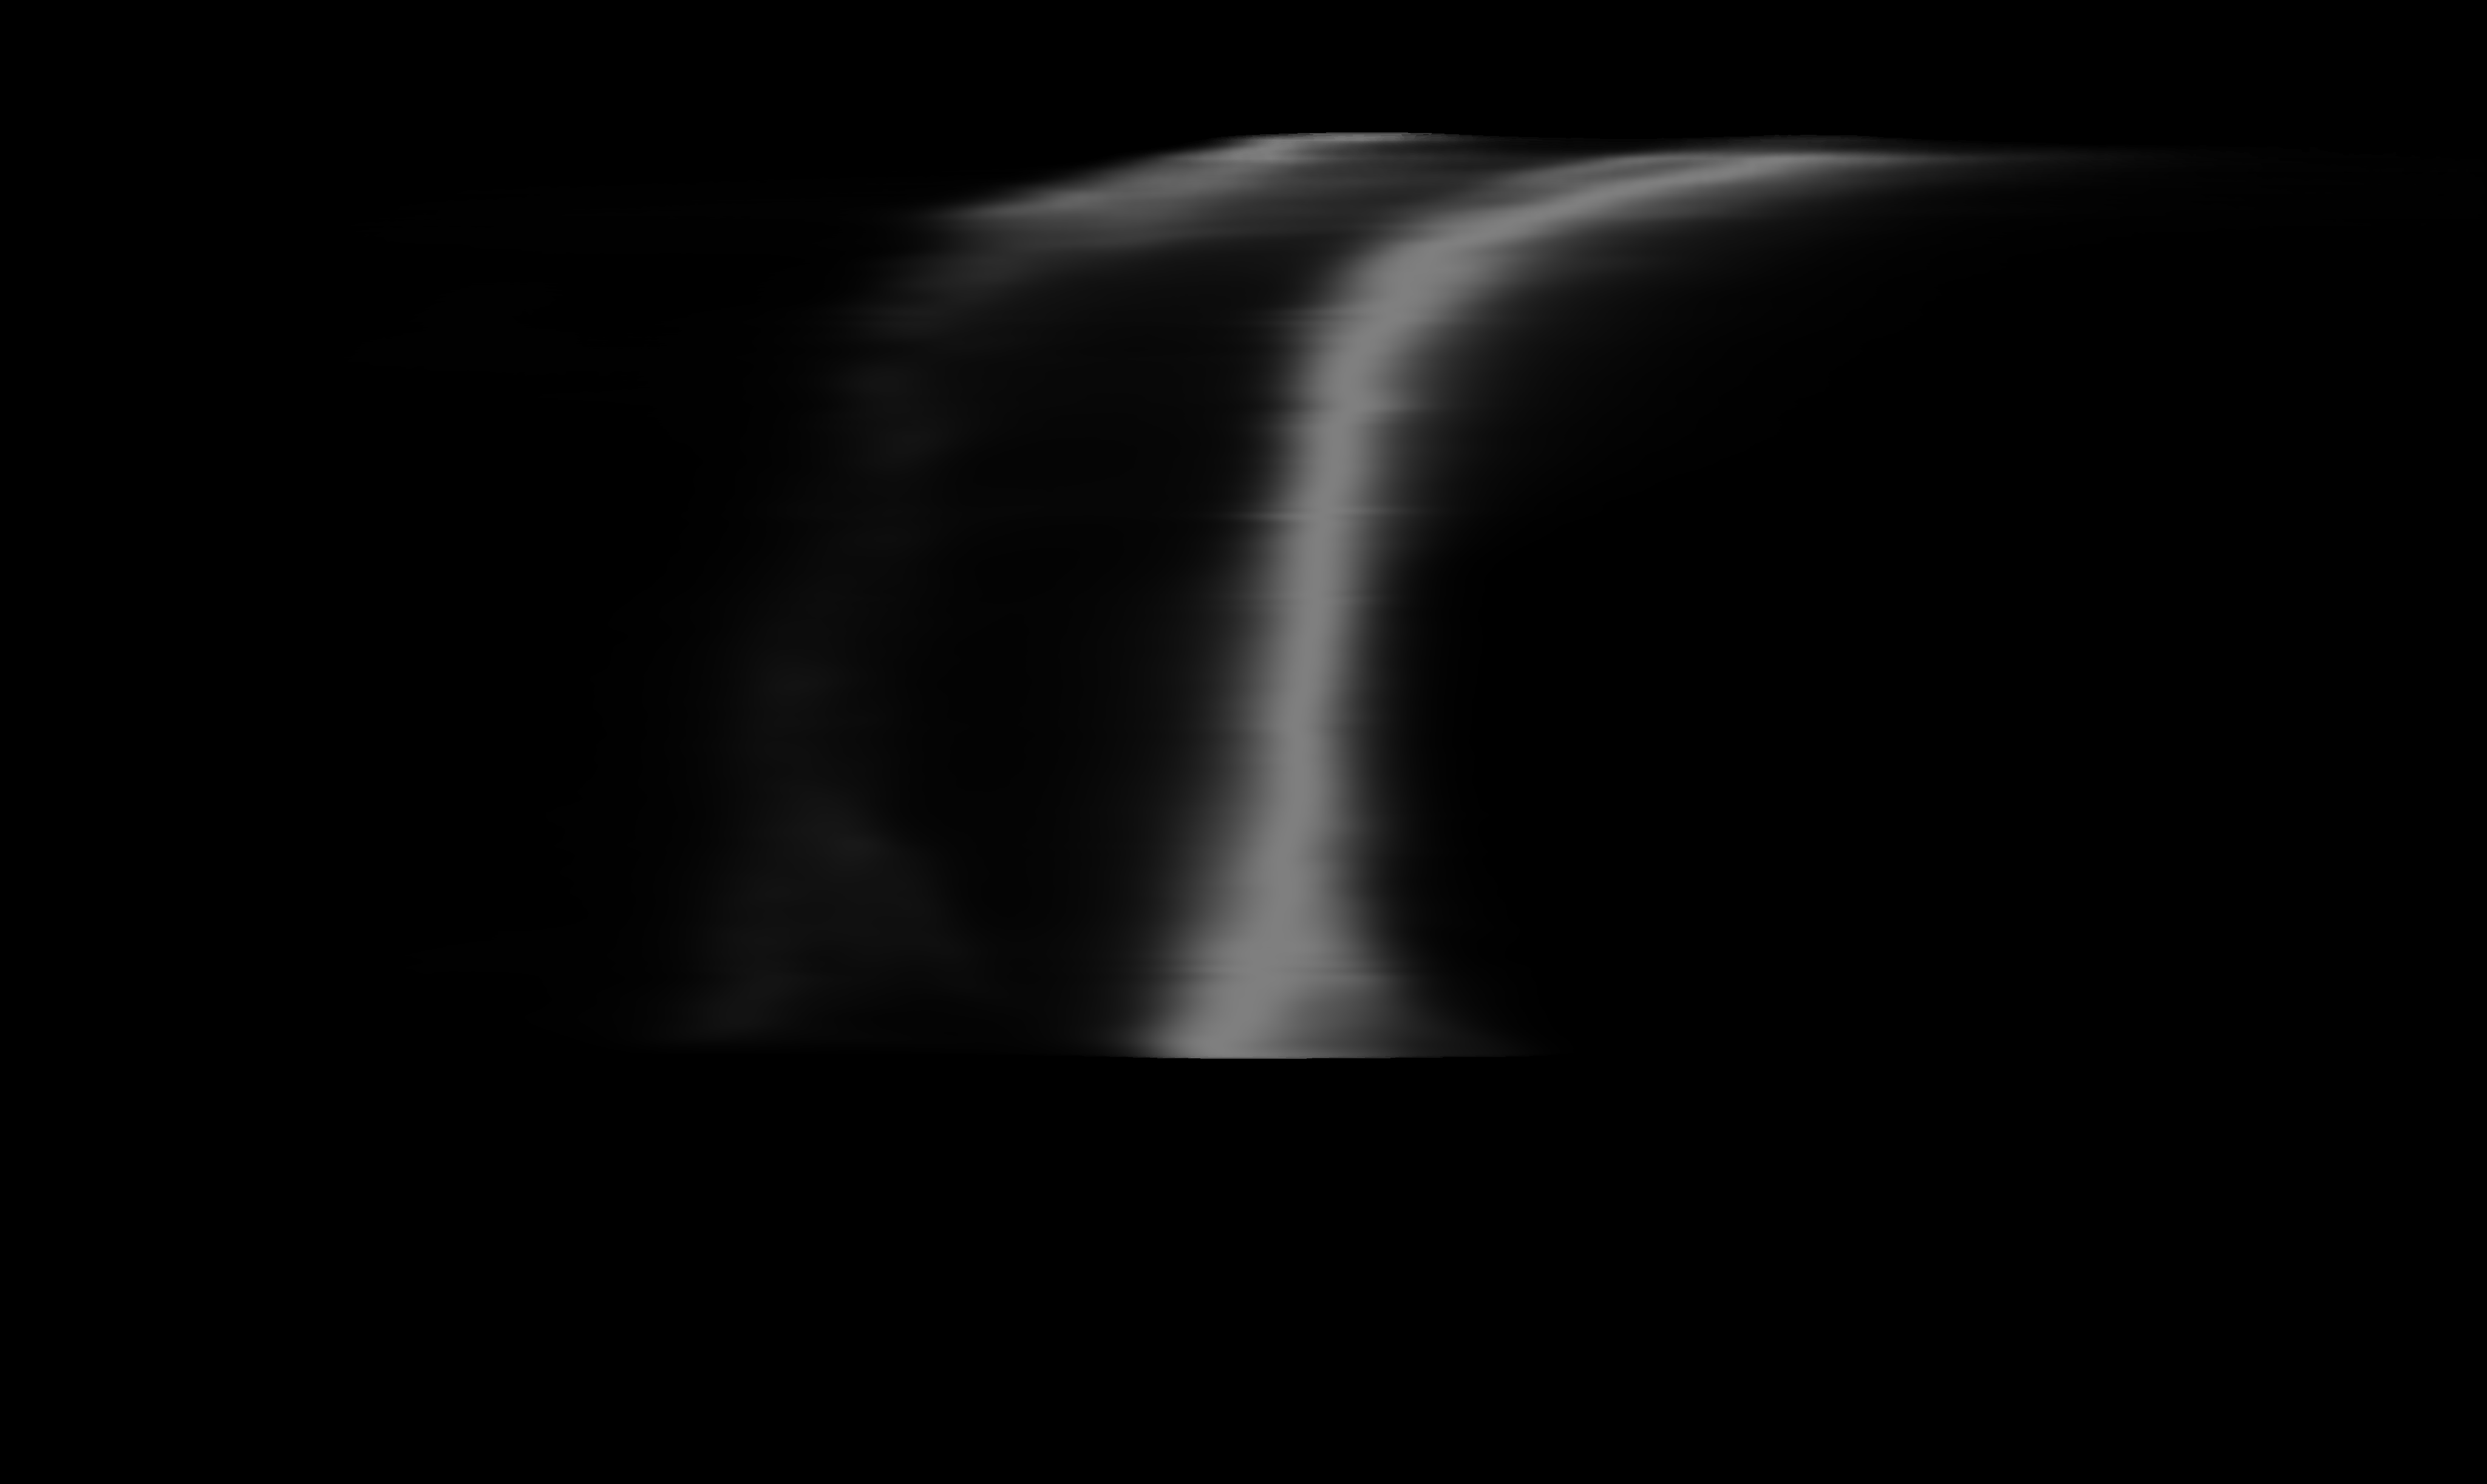
\includegraphics[width=\linewidth]{rb-bone_region3.png}
    \begin{tabular}{cc}
      \!\!\!\!\!\!(a) \begin{tabular}{c}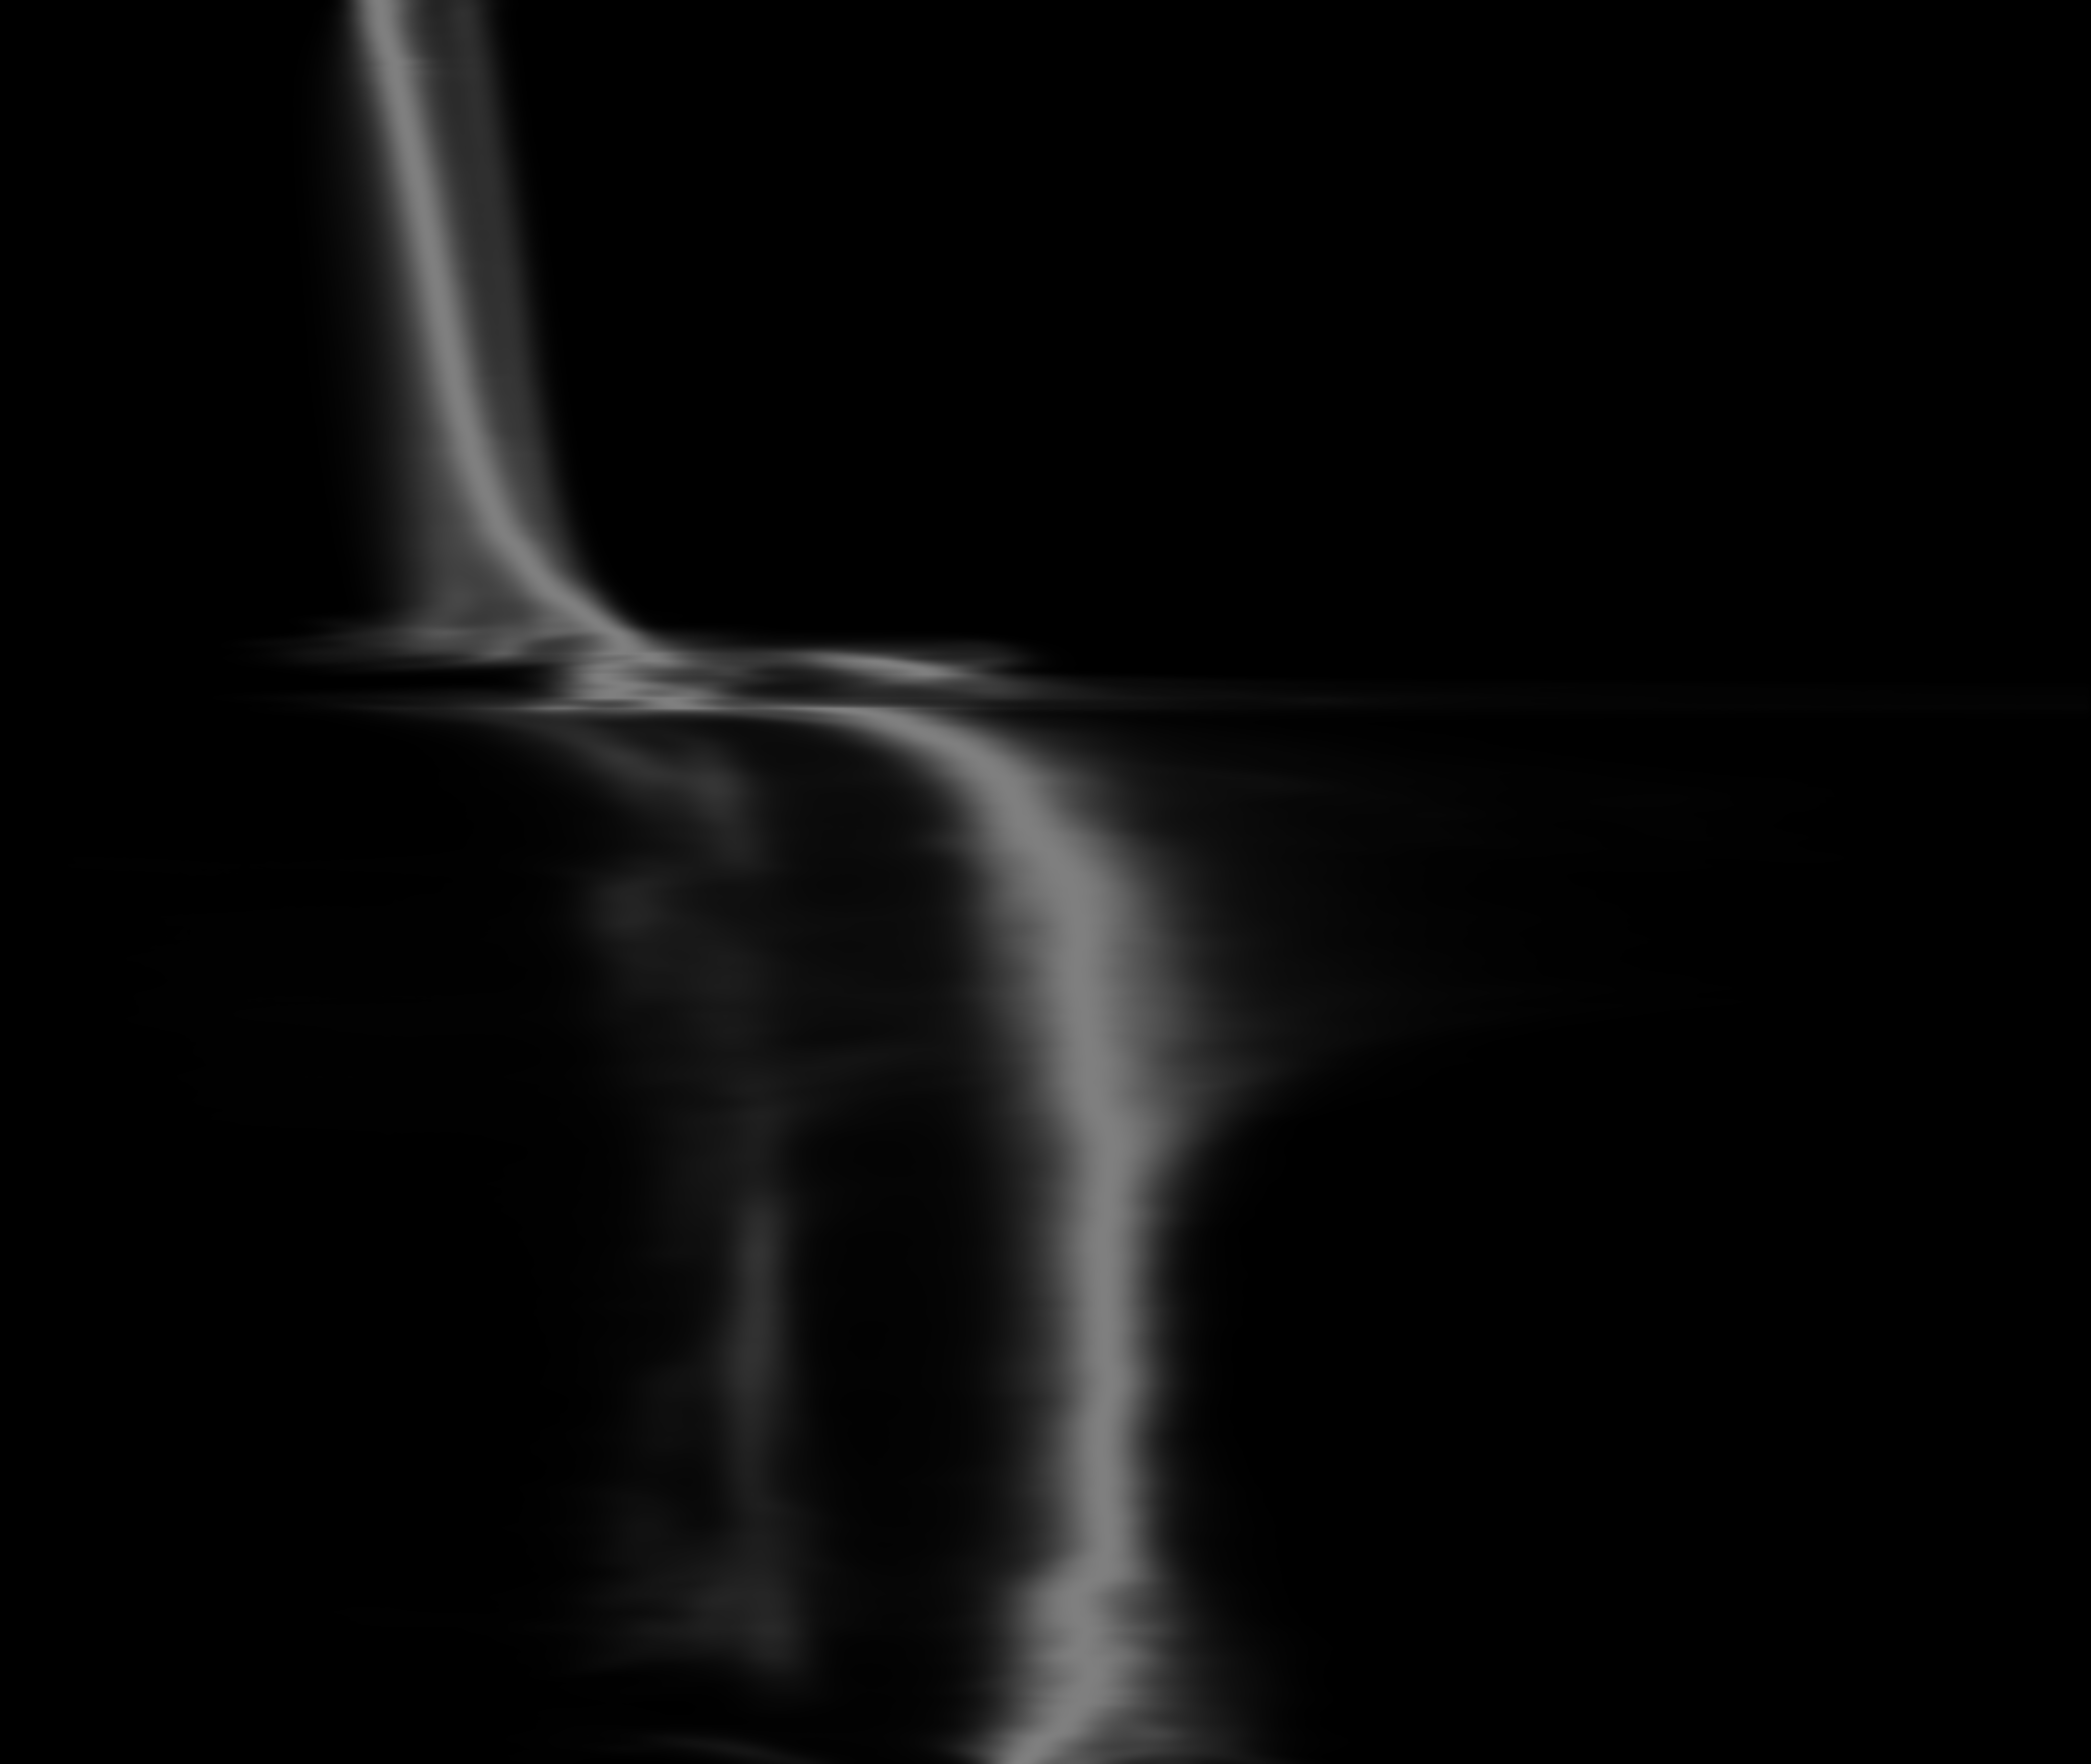
\includegraphics[width=0.96\columnwidth]{yb-full3.png}\end{tabular}\\
      \!\!\!\!\!\!(b) \begin{tabular}{c}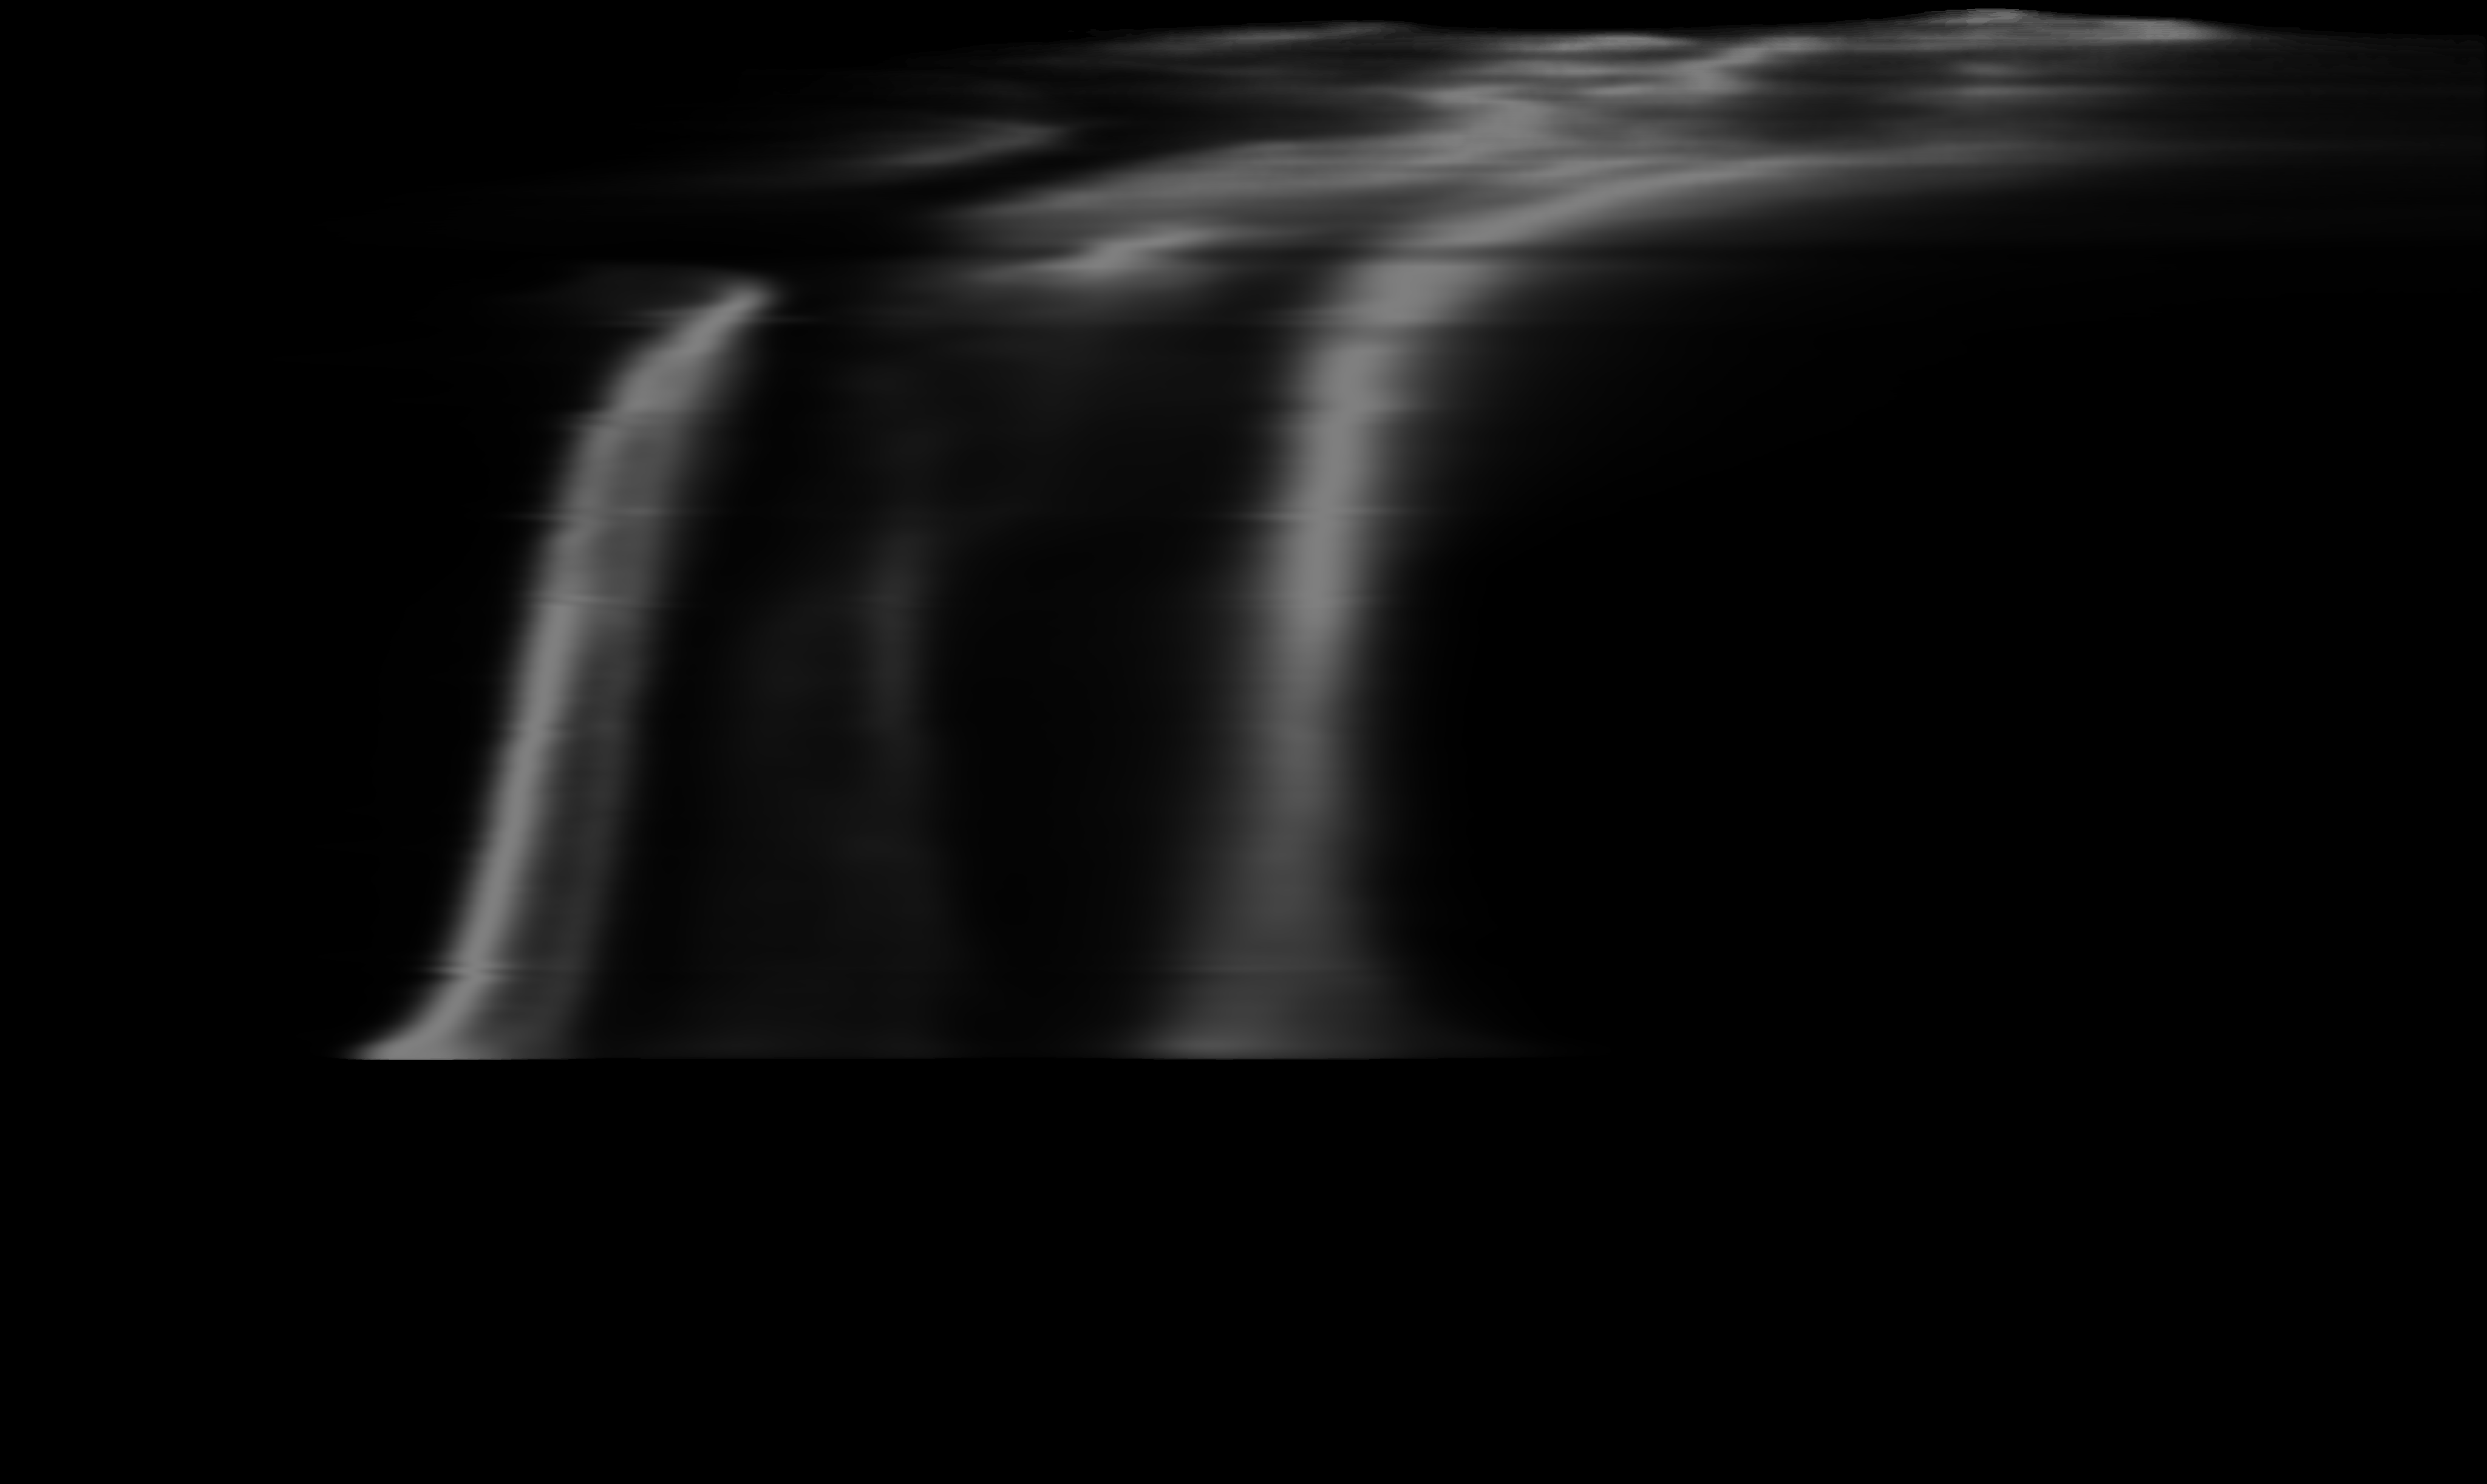
\includegraphics[width=0.96\columnwidth]{rb-full3.png}\end{tabular}\\
      \!\!\!\!\!\!(c) \begin{tabular}{c}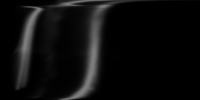
\includegraphics[width=0.96\columnwidth]{fb-edt-full2.png}\end{tabular}\\                        
%      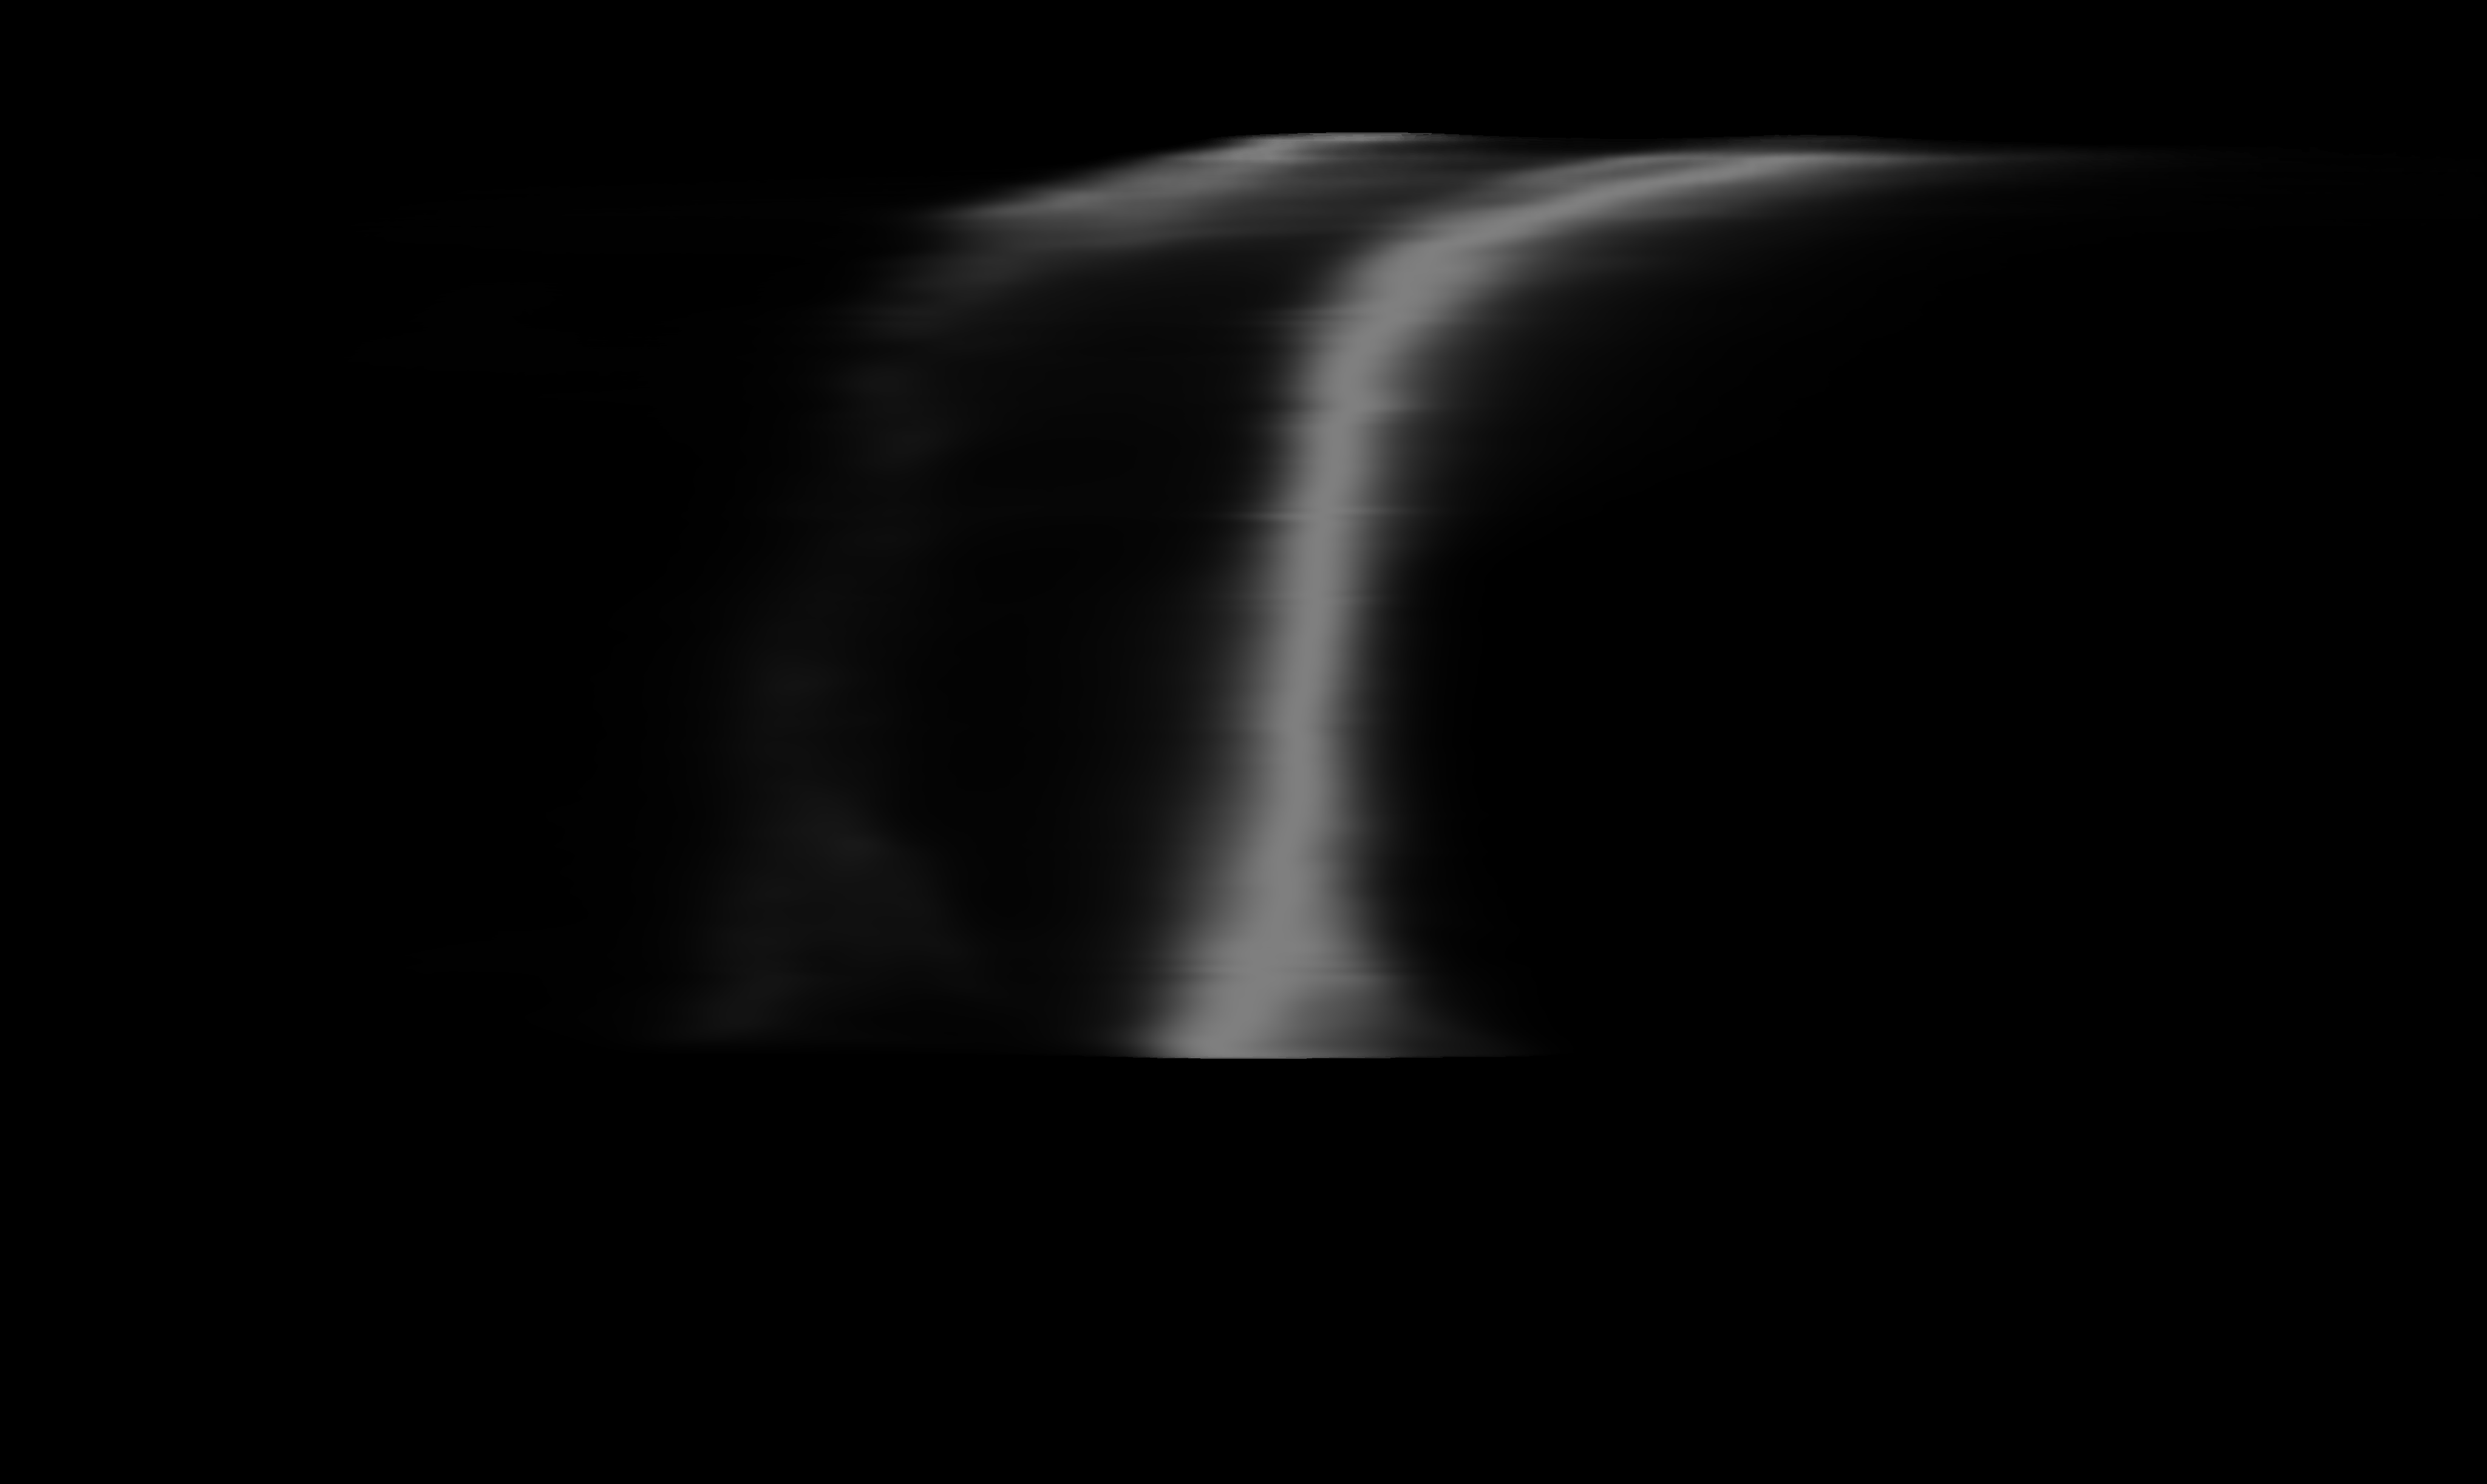
\includegraphics[width=\linewidth]{rb-bone_region3.png}\\      
    \end{tabular}
    \caption{Examples of 2D histograms for the full tomogram: (a) along the $y$-axis, (b) as a function of
      distance $r$ to the center, and (c) as a function of distance $d$ to the implant. The abscissa of the 2D histograms is voxel value, the ordinate is the value
      of $y$ resp.~$r$ and $d$. Notice that the $r$-2D histogram well separates the materials for large
      and intermediate values of $r$, but breaks down for small $r$. However, it clearly shows a brightening
      trend for small $r$. 
    }

    \label{fig:2dhists}
\end{figure}

\subsection{Field histograms}
%Show that the fields can perfectly separate
%discuss all the way to implant contact
In the present work, the main distortion we want to invert is the brightening of voxels near the high-contrast interface between
titanium implant and biological tissue, in order to accurately determine tissue-implant contact.
To this end, we can group the voxels according to their distance to the implant using the
{\em Euclidean Distance Transform} (EDT). \Cref{fig:2dhists}(c) shows the corresponding 2D histogram, which shows a darkening effect for large distances
(near the sample surface) and brightening for small distances (near the implant surface).

%EDT is good overall, but difficult close to the implant.
However, we can do better: As discussed in~\Cref{sec:physics}, the implant produces a \textit{glowing} effect, which
can be modeled physically by diffusion. \Cref{fig:edt-vs-diffusion} shows
how a voxel inside the troughs of the threading receives brightening contributions from many sides, while a voxel above the peak of the threading at
the same distance from the implant receives much less. To resolve brightening of voxels very close to the implant, it thus makes sense
to use a diffusion field, as shown in \Cref{fig:field-slice}. 


%TODO: Figuren er forkert (blå pile viser ikke afstand).
\begin{figure}
    \vspace{-1.5cm}
    \centering
    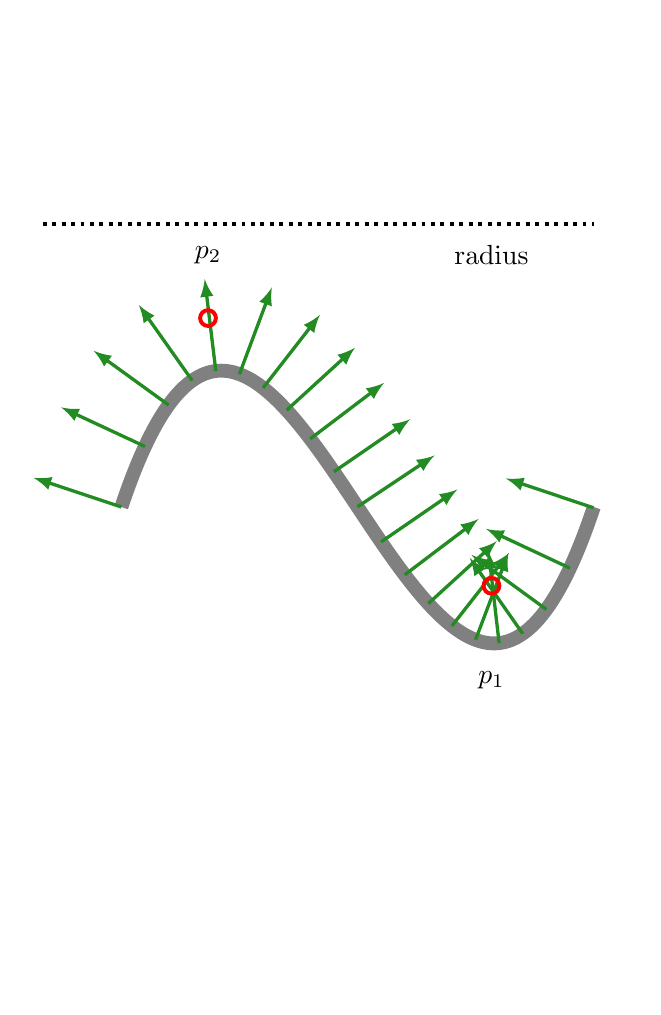
\begin{tikzpicture}[scale=2.0]
        \draw[gray,line width=5pt] (0,0)
        .. controls (1,3) and (2,-3) .. (3,0)
        \foreach \p in {0,5,...,100} {
          node[sloped,inner sep=0cm,above,pos=\p*0.01,
          anchor=south,
          minimum height=1.0cm,minimum width=1.0cm]
          (N \p){}
        }
        \foreach \p in {0,5,...,100} {
          node[midway,above,inner sep=0cm,above,pos=\p*0.01,
          anchor=south,
          minimum height=1.0cm,minimum width=1.0cm]
          (N2 \p){}
        }
        ;
        \foreach \p in {0,5,...,100} {
          \draw[-latex,ForestGreen, very thick] (N \p.south) -- (N \p.north);
%          \draw[-latex,blue,densely dotted, very thick] (N2 \p.south) -- (N2 \p.north);
        }
        \draw[red, line width=0.5mm] (0.55,1.20) circle (0.05cm);
        \node at (0.55,1.60) {$p_2$};
        \draw[red, line width=0.5mm] (2.35,-0.5) circle (0.05cm);
        \node at (2.35,-1.10) {$p_1$};
        \draw[black, line width=0.5mm, dotted] (-0.5,1.8) -- (3.0,1.8);
        \node at (2.35,1.60) {radius};
      \end{tikzpicture}
      \vspace{-3.5cm}
      \caption{Visualization of glowing effect close to the implant surface, shown in the YZ plane. 
        The two points $p_1$ and $p_2$, marked in red, have the same distance to the implant, but receive markedly different brightening effect.
        Diffusion is depicted in green, where we see multiple arrows contributing to the value of $p_1$. The dotted line depicts a constant radius from the tomogram center.}
    \label{fig:edt-vs-diffusion}
\end{figure}


\begin{figure}
    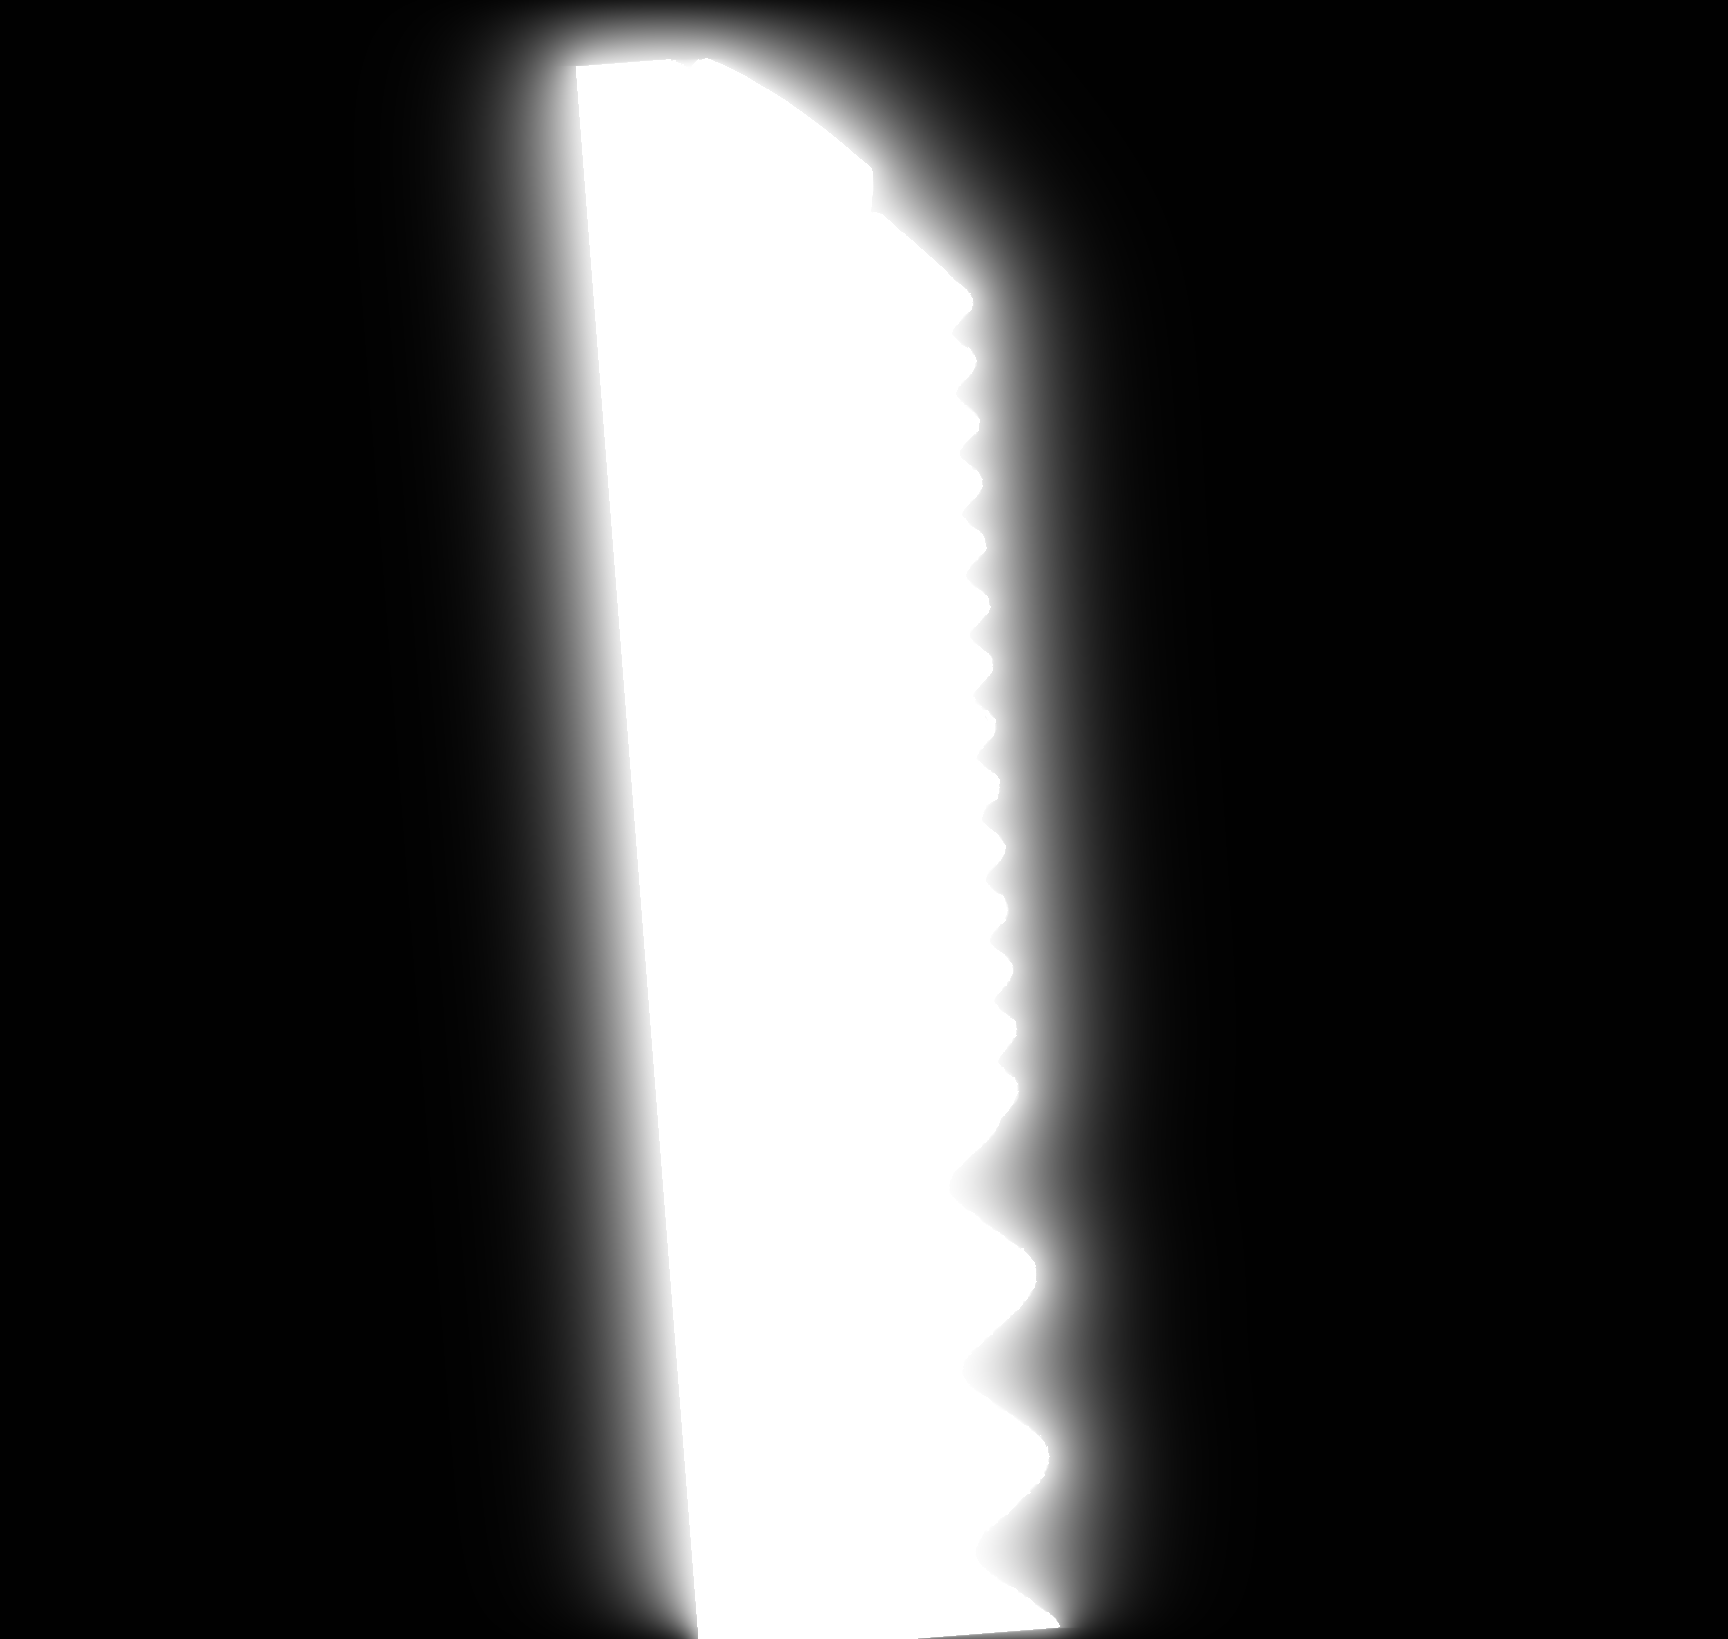
\includegraphics[width=\linewidth]{770c_pag-gauss-yz.png}
    \caption{A slice of the diffusion field in the YZ plane.}
    \label{fig:field-slice}
\end{figure}

Using a diffusion field to model the glow from the implant, we are able to describe the brightening effect even very close to the implant, but the field is nearly
zero everywhere else. In order
to construct a single field that separates voxels well according to the major contributions of distortion, we construct a combined EDT+diffusion field. We will see
in the next section that this is enough to produce a high-quality segmentation throughout the tomogram, both near the implant surface and far away from it.


% Show that the distance to the implant in edt will be the same in the grooves of the screw compared
% to the threads of the screw. This is "fixed" with diffusion, as the grooves will be brighter as it
% is surrounded by more implant.

%TODO: Adskil METODE, altsaa SASS, fra ANVENDELSE, altsaa BIC. 
\subsection{Walkthrough of the method}
This section will describe each step of our method in detail. Going from tomography to a segmented tomography.

\subsubsection{Overview}
%Coarse steps, explain the idea
In order to reach the tissue-bone implant contact metric, we have the three coarse steps: compute the fields, segmentation using the fields, and extraction of the contact from the segmented tomography.

The steps of the field computation are:
\begin{enumerate}
    \item Compute the EDT and Diffusion fields to give each voxel spatial information about its relation to the implant.
    \item Compute frequency distributions of voxel values as functions of field values as 2D histograms.
\end{enumerate}
    
Then, in order to segment using the fields:
\begin{enumerate}
    \item[3] Find the material ridges within the 2D histograms, using image processing techniques.
    \item[4] From the ridges, compute initial approximate frequency distributions of each material, which are then optimized to fit the 2D histograms.
          From the optimized distributions, we derive probability distributions for material classification. These distributions approximate the conditional probabilities $P(m|v,x)$ that a particular voxel belongs to material $m$ given that it has voxel value $v$ and field value $x$.
    \item[5] Apply the probability distributions to the tomography, segmenting the voxels into the different materials.
\end{enumerate}
    
In the present paper, we use the improved segmentation to evaluate bone-implant contact and blood-implant contact.
\begin{enumerate}
\item[6] From the segmented tomography, we compute the network of blood vessels and the osteocyte network. Voxels are classified as bone, if they are in a connected compentnt of bone-mineral and within a maximal distance from blood supply and osteocytes.
\item[7] Perform the tissue-to-implant contact analysis.
\end{enumerate}

These steps are also summarized in the flow chart in~\Cref{fig:flowchart}.

\begin{figure}
    \centering
    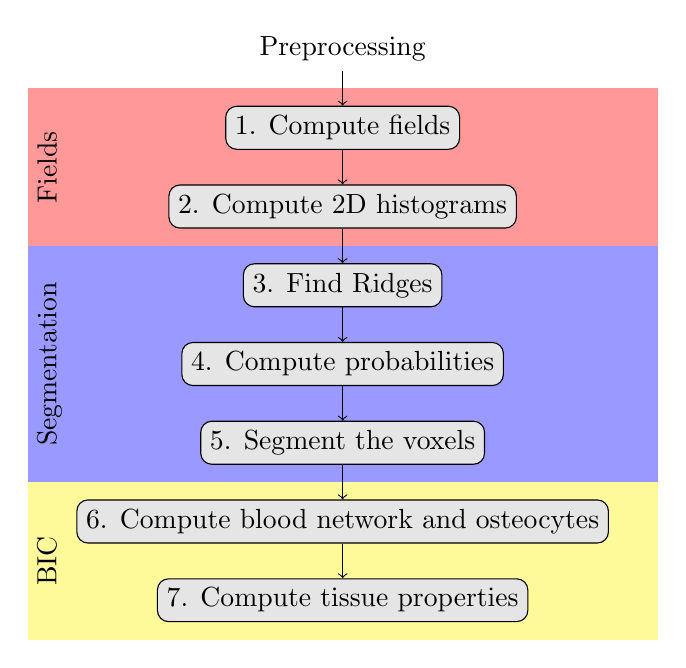
\begin{tikzpicture}
        \fill[red!40] (-4,.5) rectangle (4,-1.5);
        \fill[blue!40] (-4,-1.5) rectangle (4,-4.5);
        \fill[yellow!40] (-4,-4.5) rectangle (4,-6.5);
        \node[rotate=90, anchor=north] (field) at (-4,-.5) {Fields};
        \node[rotate=90, anchor=north] (segment) at (-4,-3) {Segmentation};
        \node[rotate=90, anchor=north] (bicc) at (-4,-5.5) {BIC};

        \node       (prep)  at (0, 1) {Preprocessing};
        \node[draw, fill=black!10, rounded corners] (field) at (0, 0) {1. Compute fields};
        \node[draw, fill=black!10, rounded corners] (hists) at (0,-1) {2. Compute 2D histograms};
        \node[draw, fill=black!10, rounded corners] (curvs) at (0,-2) {3. Find Ridges};
        \node[draw, fill=black!10, rounded corners] (probs) at (0,-3) {4. Compute probabilities};
        \node[draw, fill=black!10, rounded corners] (segm)  at (0,-4) {5. Segment the voxels};
        \node[draw, fill=black!10, rounded corners] (blood) at (0,-5) {6. Compute blood network and osteocytes};
        \node[draw, fill=black!10, rounded corners] (bic)   at (0,-6) {7. Compute tissue properties};

        \path[draw, ->] (prep)  -- (field);
        \path[draw, ->] (field) -- (hists);
        \path[draw, ->] (hists) -- (curvs);
        \path[draw, ->] (curvs) -- (probs);
        \path[draw, ->] (probs) -- (segm);
        \path[draw, ->] (segm)  -- (blood);
        \path[draw, ->] (blood) -- (bic);
    \end{tikzpicture}
    \caption{Flowchart depicting the steps of the method.}
    \label{fig:flowchart}
\end{figure}

\subsubsection{Segmentation}
The overall segmentation is computed in steps 1-5. For each step we will describe the process, showing
the algorithm where applicable, along with the the intermediate results.

\vspace{\baselineskip}
\noindent\textit{\textbf{Step 1: Field computations}}\\
Both fields are computed from the implant mask, as described in~\Cref{sec:preprocess}.
EDT is computed in parallel using W.~Silversmith's implentation of Meijster's algorithm \cite{pypi-edt},
% the Python package \texttt{edt}~\cite{pypi-edt}. %Den er implementeret i C++
yielding a 3D in which every non-implant voxel becomes the Eucledian distance of the nearest implant voxel.

For diffusion, rather than solving a full diffusion equation, we approximate it using repeated convolutions
of a 3D-Gaussian kernel, implemented by separating into 1D convolutions, as seen in~\Cref{alg:diffusion}, and the XZ-plane in~\Cref{fig:field-slice}.

\begin{algorithm}
    \caption{Diffusion approximation.}
    \label{alg:diffusion}
    \begin{algorithmic}
        \Function {Diffusion} {$voxels[n_z*n_y*n_x]$, $repitions$, \newline \indent \indent $kernel[2*k+1]$}
            \State $S \gets [n_y * n_x, n_x, 1]$
            \State $N \gets [n_z, n_y, n_x]$
            \State $buf_0[:] \gets voxels[:]$
            \For {$rep$ \textbf{in} $repitions$}
                \For {$dim$ \textbf{in} $dimensions$}
                    \For {$z,y,x$ \textbf{in} $0{:}n_z,0{:}n_y,0{:}n_x$}
                        \State $X \gets [z,y,x]$
                        \State $i_{start} \gets - \min (k, X[dim])$
                        \State $i_{end} \gets \min (k, N[dim] - X[dim] - 1)$
                        \State $i_{global} \gets z*S[0] + y*S[1] + x*S[2]$
                        \For {$i$ \textbf{in} $i_{start}:i_{end}$}
                            \State $i_{offset} \gets i_{global} + i*S[dim]$
                            \State $buf_1[index] \gets buf_0[i_{offset}] * kernel[i+k]$
                        \EndFor
                    \EndFor
                    \State $buf_0[:] \gets buf_1[:]$
                \EndFor
            \EndFor
            \Return $buf_0$
        \EndFunction
    \end{algorithmic}
\end{algorithm}

%EDT + Diffusion
To obtain a good separation both close to the implant and far away, we combine the two fields into a
single one as shown in~\Cref{eq:field-comb}.

%\begin{algorithm}
%    \caption{Field combination}
%    \label{alg:field-comb}
%    \begin{algorithmic}
%        \Function {field\_combine} {$f_{edt}, f_{dif}$}
%            \State $r \gets f_{dif} - \frac{f_{edt}}{\max (f_{edt})}$
%            \State $r \gets r - \min (f_{dif})$
%            \State $r \gets \frac{r}{\max (f_{dif})}$
%
%            \Return $r$
%        \EndFunction
%    \end{algorithmic}
%\end{algorithm}

\begin{equation}
    \label{eq:field-comb}
    \begin{split}
        f_{combined} &= \frac{f_{diffusion} - \frac{f_{edt}}{\max (f_{edt})} \min (f_{diffusion})}{\max (f_{diffusion})}
    \end{split}
\end{equation}

\vspace{\baselineskip}
\noindent\textbf{Step 2: 2D histograms} \\
From the combined fields we compute a 2D-histogram with the field value on the y-axis and the voxel
value on the x-axis.  The algorithm for the field-histogram can be seen in~\Cref{alg:field-hist}
along with a plot of the resulting histogram in~\Cref{fig:field-hist}. We see that the bone and soft tissue
separate neatly into two distinguishable distributions. The effect of the diffusion field is to ``zoom in'' near the implant surface,
where the diffusion field changes rapidly.


\begin{algorithm}
    \caption{Field 2D histograms.}
    \label{alg:field-hist}
    \begin{algorithmic}
        \Function {Field\_hist} {$voxels[n_z,n_y,n_x]$, $field[n_z,n_y,n_x]$, $v_{bins}$, \indent \indent $v_{min}$, $v_{max}$, $f_{bins}$, $f_{min}$, $f_{max}$}
            \For {$z,y,x$ \textbf{in} $0{:}n_z,0{:}n_y,0{:}n_x$}
                \State $v \gets voxels[z,y,x]$
                \If {$v_{min} \leq v \leq v_{max}$}
                    \State $f \gets voxels[z,y,x]$
                    \If {$f_{min} \leq f \leq f_{max}$}
                        \State $v_i \gets (v_{bins} - 1) - \frac{v - v_{min}}{v_{max} - v_{min}}$
                        \State $f_i \gets (f_{bins} - 1) - \frac{f - f_{min}}{f_{max} - f_{min}}$
                        \State $h[f_i,v_i]{+}{+}$
                    \EndIf
                \EndIf
            \EndFor
            \Return $h$
        \EndFunction
    \end{algorithmic}
\end{algorithm}

\begin{figure}
    %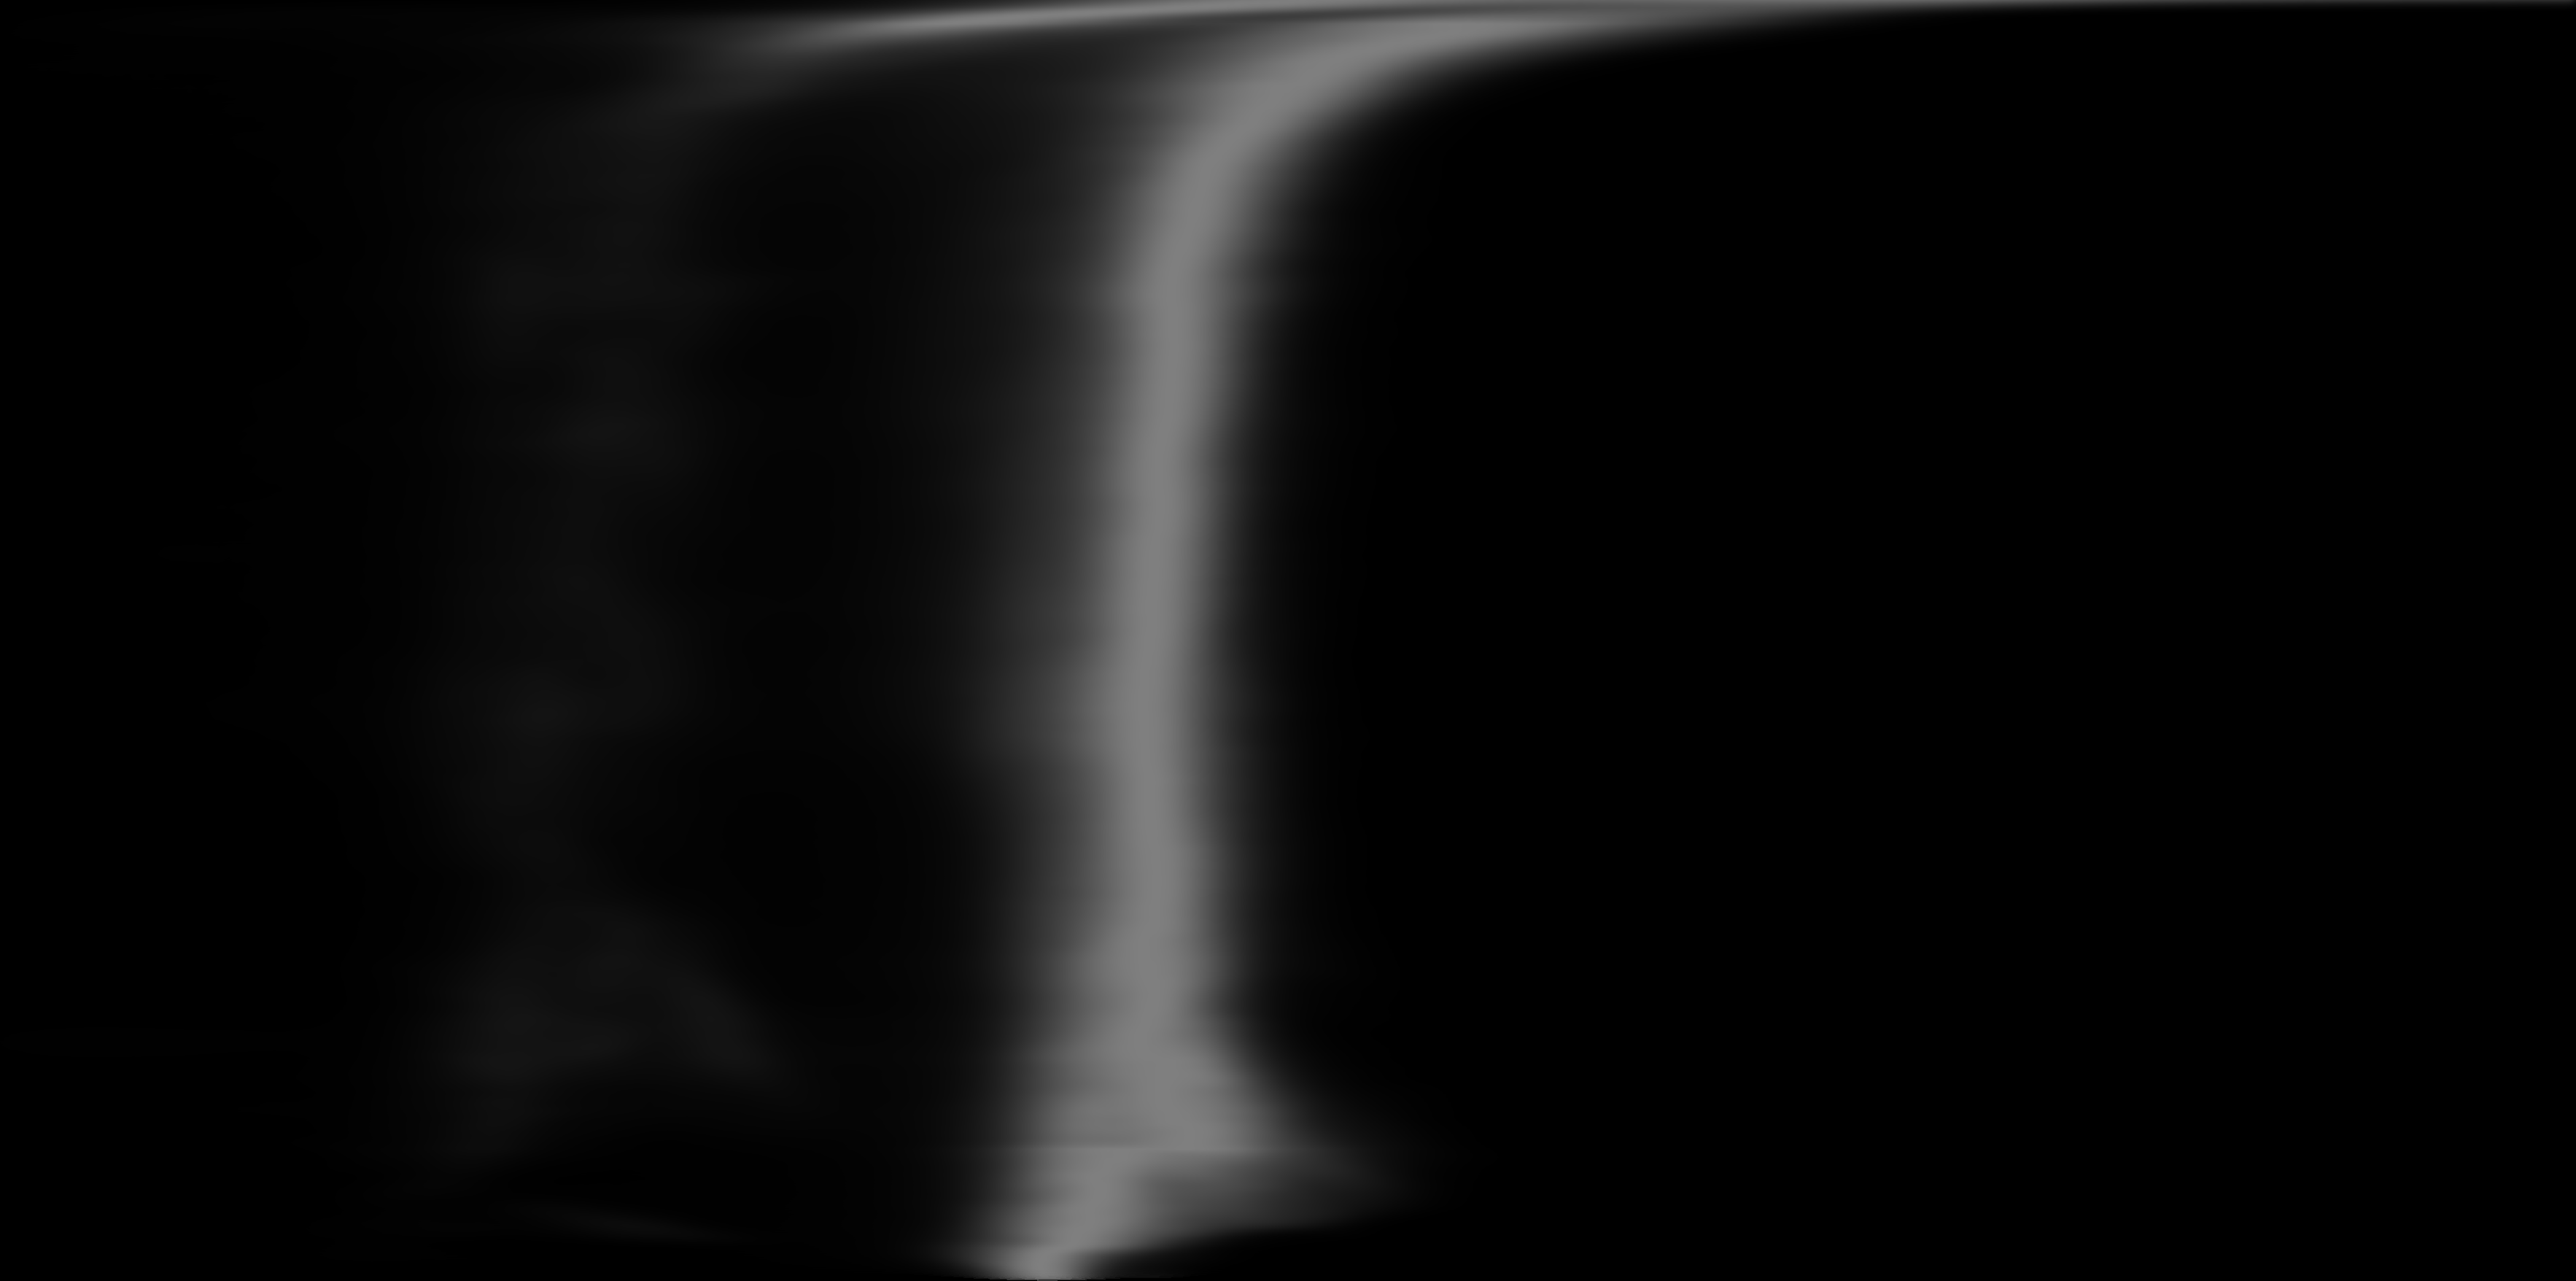
\includegraphics[width=\linewidth]{fb-edt-bone_region3.png}
    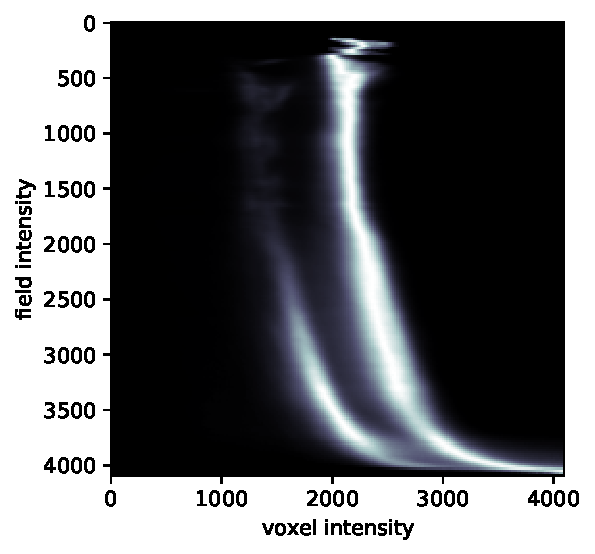
\includegraphics[width=\linewidth]{fb-gauss+edt-bone_region3.pdf}
    \caption{2D field histogram. Note that there are two clearly separated ridges, which each represent
      the expectation value for a particular material as a function of the field value.}
    \label{fig:field-hist}
\end{figure}

\vspace{\baselineskip}
\noindent\textbf{Step 3: Identify the materials} \\
In order to decompose 2D histogram into a sum of probability distributions that represent
the different materials present in the tomogram, we first identify the {\em ridges}:
i.e., the peaks in the 1D histograms that are persistent and vary continuously with the field value.
Thus we can expect each ridge to represent the {\em expectation values} for a particular material
as a function of the field value, i.e., as a function of the voxel's position in space.

Any ridge-finding method will do: we compute it through the series of image processing operations shown in
\Cref{alg:material}.
% The next step is to isolate the different materials spatially, which is done through the field-histogram.
% For our first attempt, we applied Otsu's threshold to each each row in the 2D-histogram. While this
% provided good results for two well defined distributions, it eventually began to fail. This was either
% because of lack of samples, or because the histogram did not contain two distributions, which is an
% underlying assumption of Otsu thresholding. These two effects occurred at the edges (both closest and
% furthest from implant), which would bleed into the later steps of the segmentation process.

% Rather than finding the threshold value in between the distributions, our next solution was to start
% finding the distributions by finding the ridges of the 2D-histogram. We do this by applying a series
% of image processing techniques, described in~\Cref{alg:material}. Each of the resulting contours
% become their own material, which are then labeled as material 1 or 2 respectively for this particular
% sample. For samples that would contain more than two distributions, the same algorithm should apply,
% as long as the distributions does not overlap.

\begin{algorithm}
    \caption{2D histogram ridge-finding.}
    \label{alg:material}
    \begin{algorithmic}
        \Function {Ridges} {$h[f_{bins}$, $v_{bins}]$, $\sigma$, $peak_{min}$, $k_x$, $k_y$, \newline \indent \indent $i_{dilate}$,$i_{erode}$, $t$}
            \For {$row$ \textbf{in} $0{:}f_{bins}$}
                \State $r \gets gaussian\_smooth(h[row,:], \sigma)$
                \State $p \gets find\_peaks(r, peak_{min})$
                \State $ps[p] \gets 1$
            \EndFor
            \State $kernel = cross\_kernel(k_x, k_y)$
            \State $d \gets dilate(ps, i_{dilate}, kernel)$
            \State $e \gets erode(d, i_{erode}, kernel)$
            \State $cs \gets find\_contours(e)$
            \For {$i$ \textbf{in} $0{:}|cs|$}
                \If {$size(cs[i]) > t$}
                    \State $l \gets draw\_contour(l, cs[i], i+1)$
                \EndIf
            \EndFor
            \Return $l$
        \EndFunction
    \end{algorithmic}
\end{algorithm}

\begin{figure*}
    % %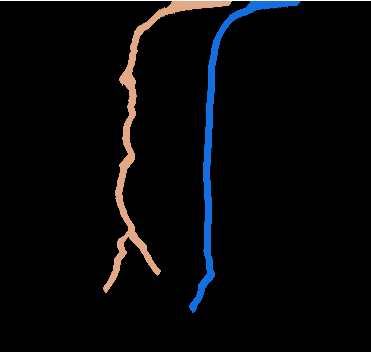
\includegraphics[width=0.5\linewidth]{curves_edt.png}%
    % %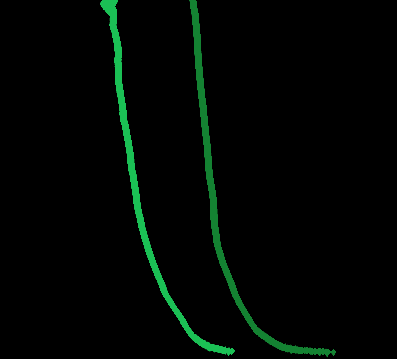
\includegraphics[width=0.5\linewidth]{curves_diffusion.png}
    % 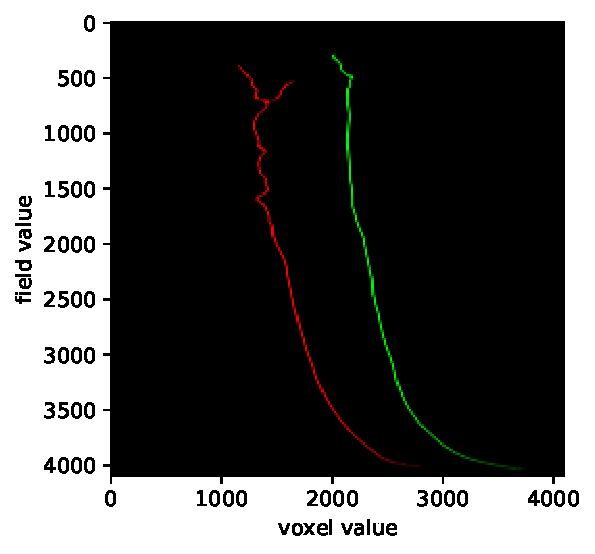
\includegraphics[width=\linewidth]{ridges_gauss+edt-bone_region3.pdf}
    % \james{will produce overall plot with probabilities}
    % \caption{Detected ridges from the combined field histogram.}
    % \label{fig:curves}
  \centering
  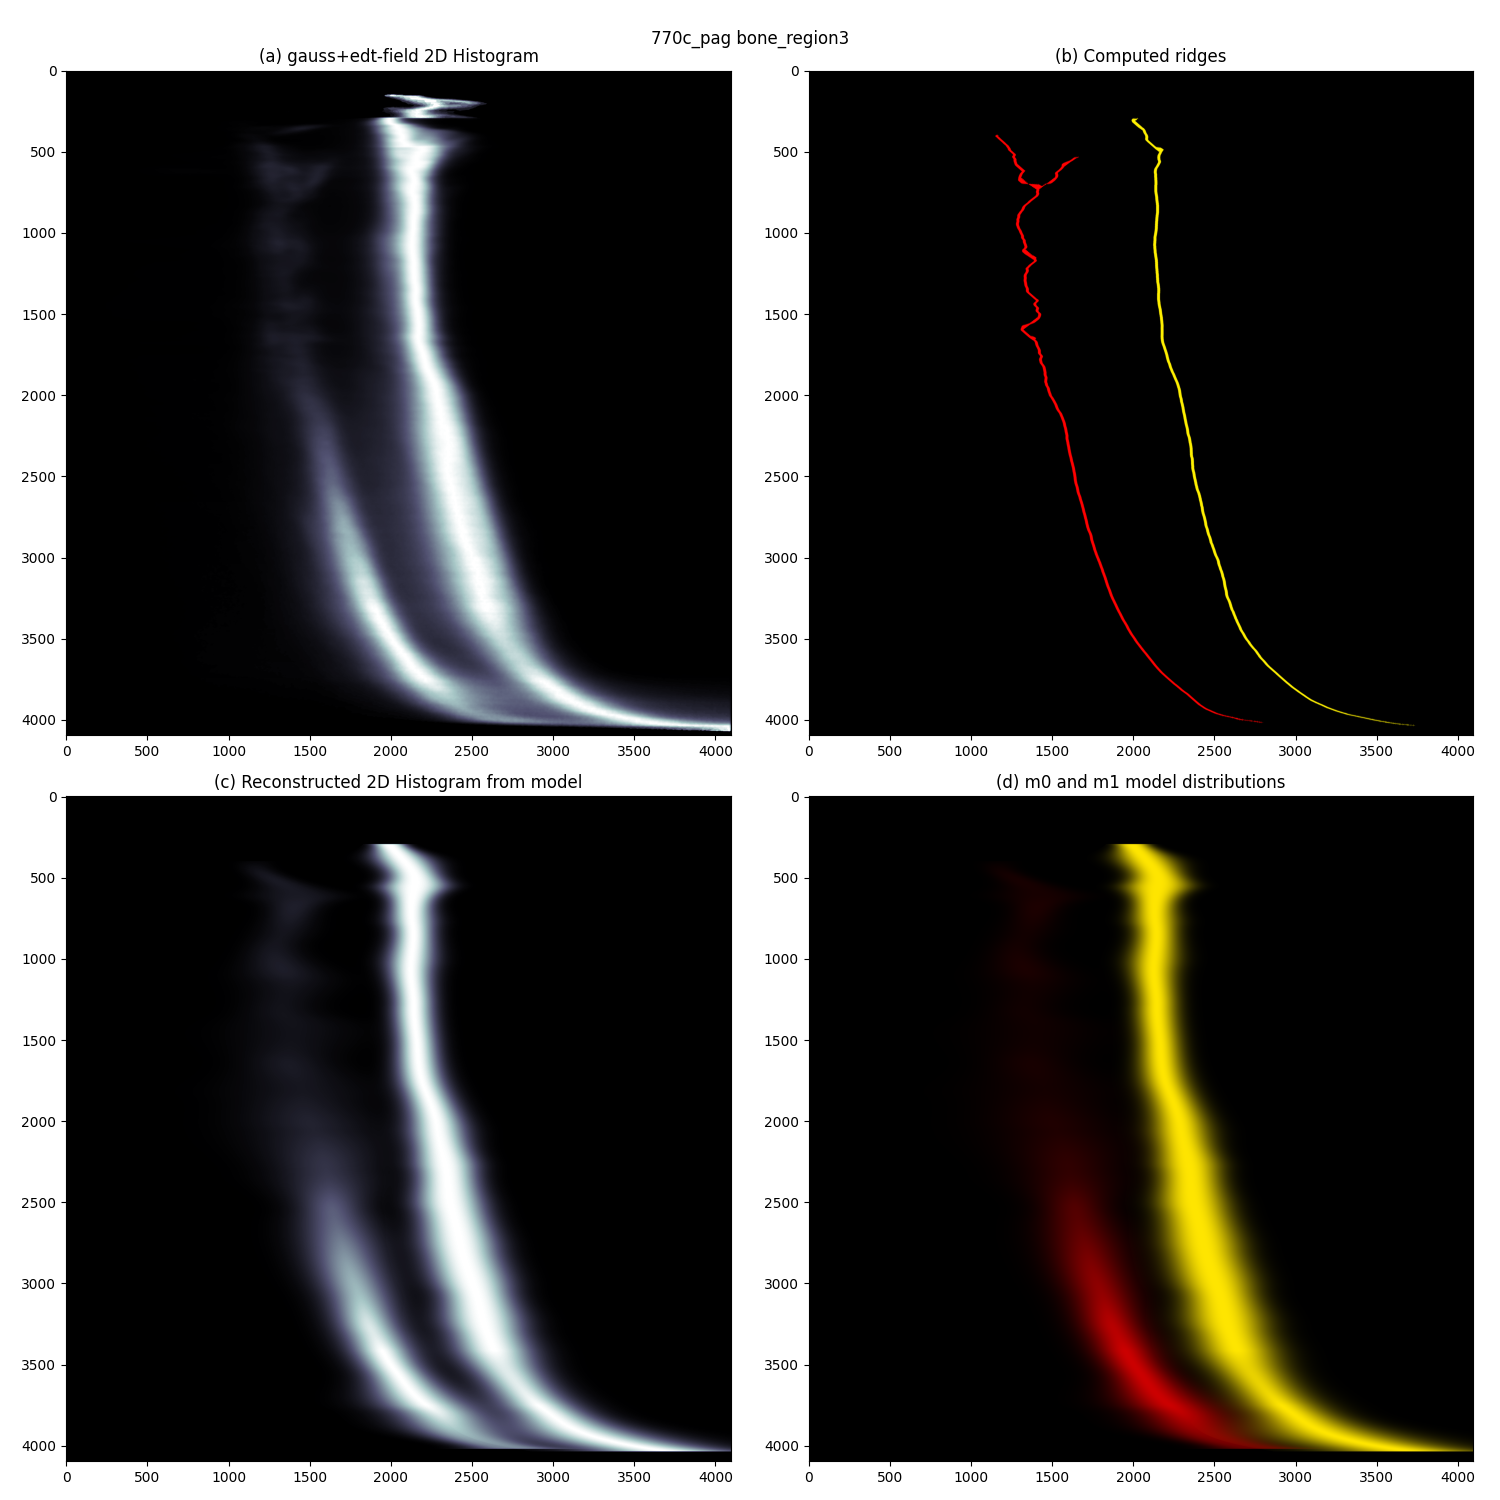
\includegraphics[width=.9\textwidth]{compute_probabilities_gauss+edt_bone_region3}\\
  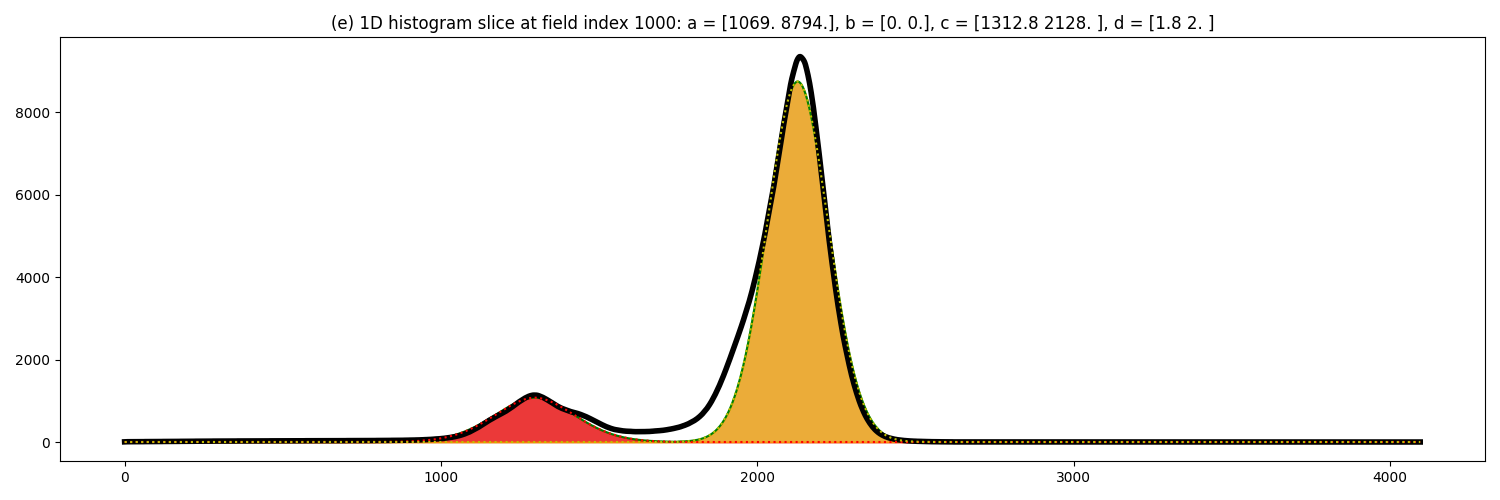
\includegraphics[width=.9\textwidth]{hist_slice_gauss+edt_bone_region3}\\
  \caption{(a) Measured 2D histogram for the compound diffusion+distance field from Step 2. (b)
    The detected ridges from Step 3. (c) Sum of computed frequency distribution models
    with optimized smooth piecewise cubic functions for parameters $a(\fval), b(\fval), c(\fval), d(\fval)$:
    this is the part of the 2D histogram explained by the smooth model. (d) The individual distributions evaluated
    on the 2D field-value$\times$ voxel-value grid. (e) A single 1D slice of the 2D histogram (black) together with
    the model frequency distributions. Red is soft-tissue, yellow is bone mineral.
  }
  \label{fig:curves-and-more}
\end{figure*}

\vspace{\baselineskip}
\noindent\textbf{Step 4: Compute models for material probability distributions} \\
Our goal is to obtain good conditional probability distributions $P(m|v,\xx)$
that model the likelihood of a voxel having material type $m$ as a function
both on its value $v$ and its position $\xx$ in space. For the probabilities
conditioned on the field values (distance or diffusion field), we model
the probability distributions $P(m|v,f(\xx))$ conditioned on
voxel- and field values. We want to make sure that these distribution
functions vary smoothly across space (or as a function of field values),
to ensure that we can identify the materials correctly across the entire
image: i.e., even though the frequency distributions look completely different
close to the titanium implant compared to the middle region or sample surface,
we can track the unbroken, smooth deformation to assign a global material
identity.

To this end, we first {\it model the frequency distributions} using the
2D histograms. Given that we are modeling materials $m=1,\ldots,M$,
we write the full 2D histogram as a sum of distributions
$g_m(\fval,v)$ modeling the described part, and an undescribed
residual $r(\xx,v)$.
\begin{equation}
  \label{eq:hist}
  H(\fval,v) = \sum_{m=1}^M g_m(\fval,v) + r(\fval,v)
\end{equation}
The residual is constrained to be non-negative, i.e., we must not explain
more voxels than the image contains.
The distribution functions can be chosen in any way that approximately
model the observed frequencies: we first used Gaussians with passable success,
but found that they dropped off too rapidly. We instead found excellent results
with the next-simplest model, leaving the exponential power free:
\begin{equation}
  \label{eq:dist-form}
  g_m(\fval,v) = a_m(\fval) e^{-b_m(\fval) |v-c_m(\fval)|^d_m(\fval)}
\end{equation}
where for each field value $\fval$
$a(\fval)$ is the distribution height at the center $v=c(\fval)$,
$b(\fval)$ is the exponential falloff rate, and $d(\fval)$ is
the exponential power ($d=2$ yields a Gaussian, $d=1$ a simple exponential).
In practice we found $1.5\le d \le 2$ to best match the actual frequency
distribution decay rates.

Using the ridges found in the previous step, we generate good starting
guesses and constraints for the distribution parameters
$a,b,c,d$:
For each field-value $\fval$ (corresponding to a row in the 2D histogram),
we initialize the starting approximation as:
\begin{equation}
  \label{eq:starting-guesses}
  \begin{split}
    c_m(\fval) &= \mathop{\mathtt{argmax}}_{v \text{ with }\lab[\fval,v] = m} H(\fval,v)    \\
    a_m(\fval) &= H(\fval,c_m(\fval))\\
    b_m(\fval) &= 3/\mathrm{width}_m(\fval)^2 \\
    d_m(\fval) &= 2
  \end{split}
\end{equation}
where we use half the distance to the center of ridge $m+1$ as the width
$\mathrm{width_m}(\fval)$, using the relation that $b = 3/w^d$ yields
a $5\%$ cutoff at $w$ when $1\le d \le 2$. This approximation
already yields a good approximation. Thus, the subsequent
optimization using the constrained quasi-Newton optimization method L-BFGS-B\cite{BFGS}
converges rapidly to an excellent fit. Each 1D histogram row is first optimized
independently in parallel: The resulting numerical functions
$a_m(\fval),\ldots,d_m(\fval)$ are then converted into piecewise cubic
functions using a least squares-based algorithm that ensures continuity
and differentiability across the piecewise segments. This lets us interpolate across
outliers due to noise, but equally important:
extrapolate our models smoothly into the regions very close to the implant, where
we don't have enough voxels to produce good statistics.

We finally obtain the {\it conditional probabilities} from the material frequency distribution
models $g_m$ as:
\begin{equation}
  \label{eq:Pm}
  P(m|v,f(\xx)) = \frac{g_m(v,f(\xx))}{H(v,f(\xx))}
\end{equation}
(well-defined where $H(v,\fval) > 0$, zero outside this region as $0\le g_m \le H$).



%%% Local Variables:
%%% mode: latex
%%% TeX-master: "main"
%%% End:


\vspace{\baselineskip}
\noindent\textbf{Step 5: Perform segmentation} \\
The final step of the segmentation process is to use the probabilities for segmentation.
This process is fairly straightforward, as each voxel is looked up in the probability distribution,
which carries the same shape as the field-histogram.

\begin{algorithm}
    \caption{Final segmentation from the probability distributions.}
    \label{alg:segment}
    \begin{algorithmic}
        \Function {Segment} {$voxels[n_z,n_y,n_x], p[f_{bins},v_{bins}],$ \newline \indent \indent $v_{bins}, v_{min}, v_{max}, f_{bins}, f_{min}, f_{max}$}
            \For {$z,y,x$ \textbf{in} $0{:}n_z,0{:}n_y,0{:}n_x$}
                \State $v \gets voxels[z,y,x]$
                \If {$v_{min} \leq v \leq v_{max}$}
                    \State $f \gets voxels[z,y,x]$
                    \If {$f_{min} \leq f \leq f_{max}$}
                        \State $v_i \gets (v_{bins} - 1) - \frac{v - v_{min}}{v_{max} - v_{min}}$
                        \State $f_i \gets (f_{bins} - 1) - \frac{f - f_{min}}{f_{max} - f_{min}}$
                        \State $result[z,y,x] \gets p[f_i, v_i]$
                    \EndIf
                \EndIf
            \EndFor
            \Return $result$
        \EndFunction
    \end{algorithmic}
\end{algorithm}

\subsection{Results of the field-segmentation}

Here we present the final output from the steps described above.

\begin{figure}
    \centering
    \begin{subfigure}[b]{\linewidth}
        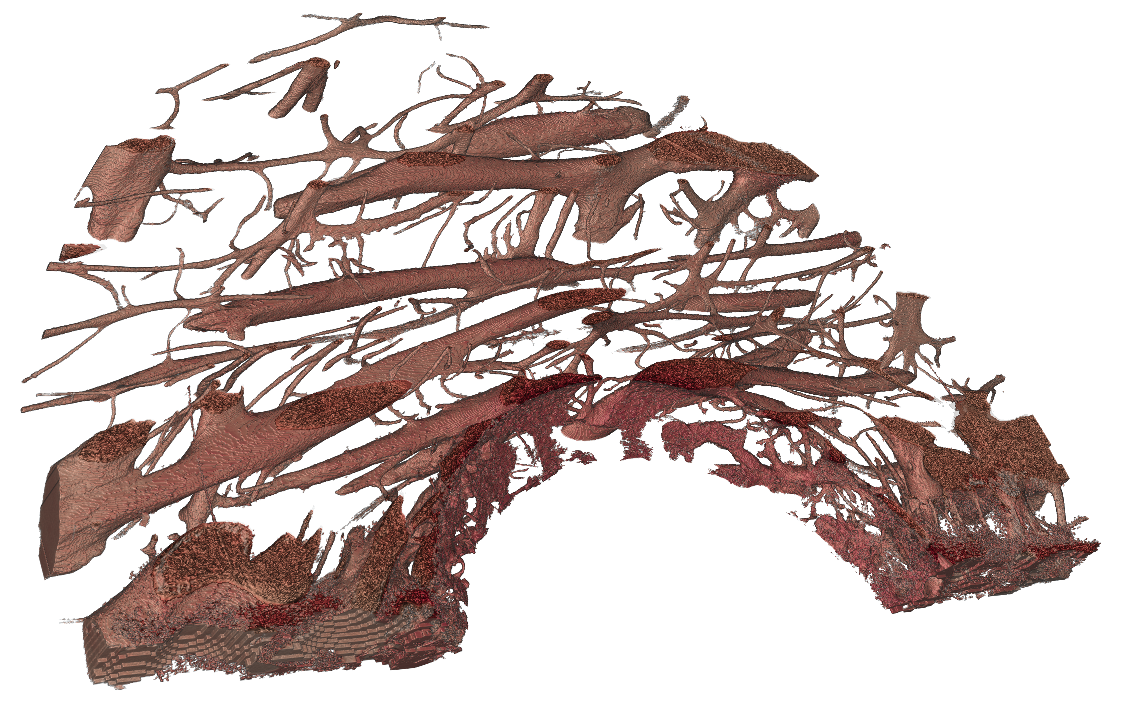
\includegraphics[width=\linewidth]{figures/blood_old_bone_100.png}
        % TODO opdater hvis en anden slice størrelse bliver brugt. voxel size = 3.75
        \caption{3D render of a $375\mu m \times 4230\mu m \times 6480\mu m$ slice of the blood network in the old bone region.}
        \label{fig:blood-old-slice}
    \end{subfigure}
    \begin{subfigure}[b]{\linewidth}
        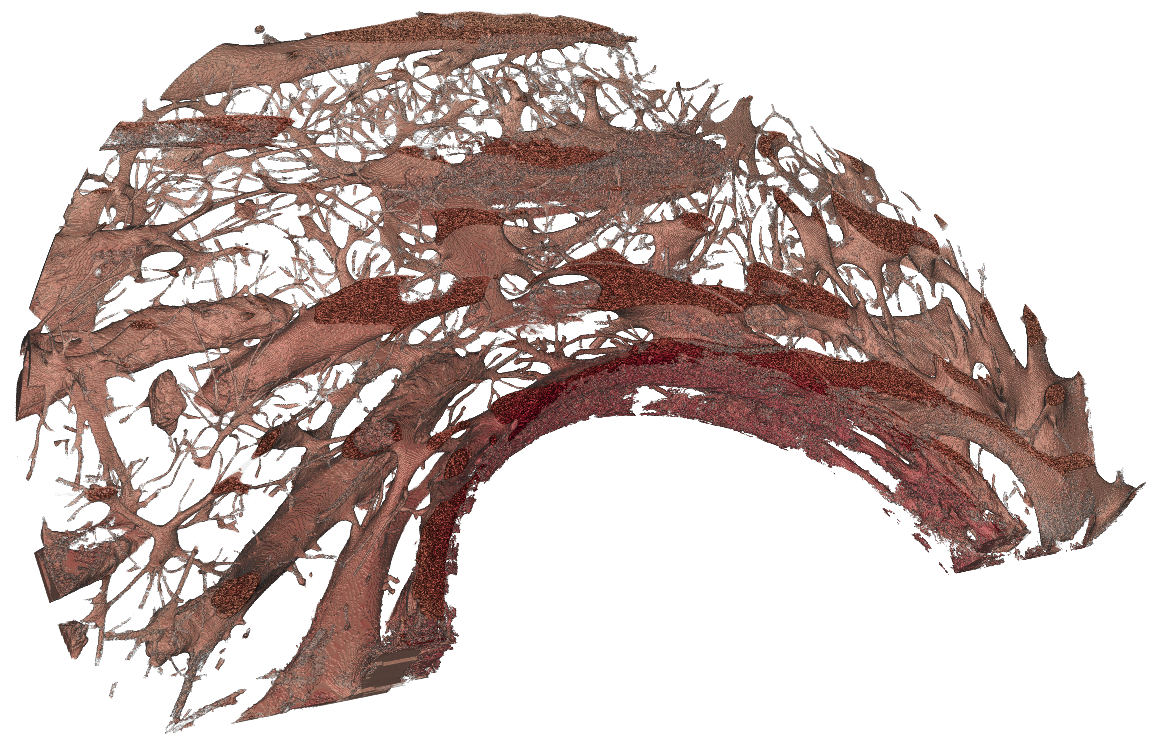
\includegraphics[width=\linewidth]{figures/blood_new_bone_100.png}
        \caption{3D render of a $375\mu m \times 4230\mu m \times 6480\mu m$ slice of the blood network in the new bone region.}
        \label{fig:blood-new-slice}
    \end{subfigure}
    \begin{subfigure}[b]{.45\linewidth}
        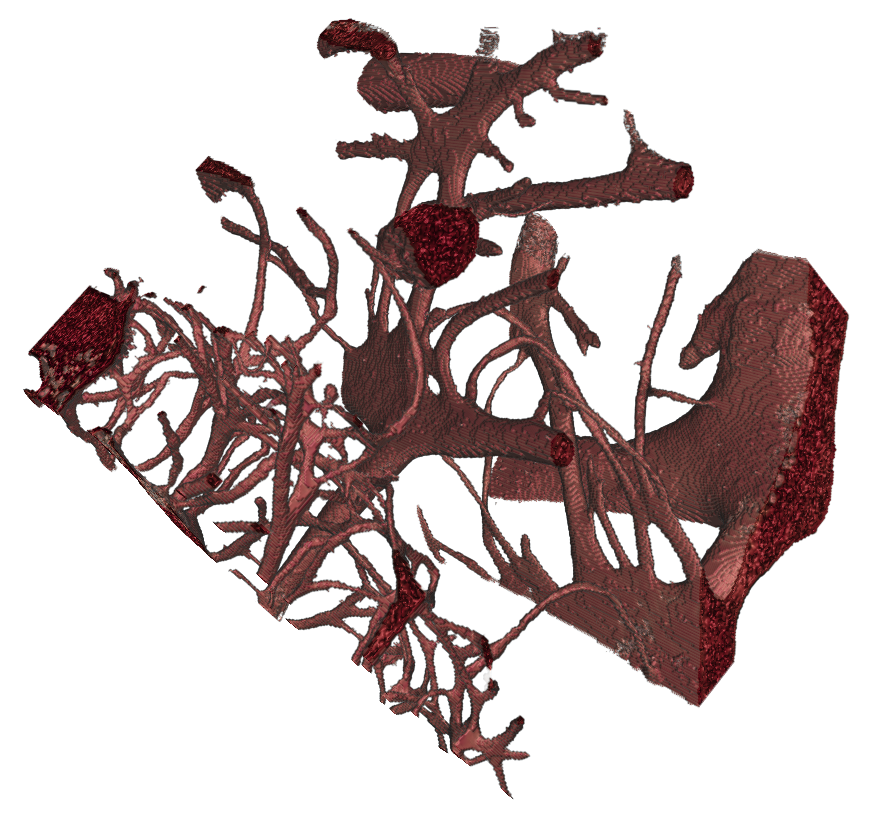
\includegraphics[width=\linewidth,height=\linewidth]{figures/blood_old_cube.png}
        \caption{3D render of a $1mm \times 1 mm \times 1 mm$ cube of the blood network in the old bone region.}
        \label{fig:blood-old-cube}
    \end{subfigure}
    \hfill
    \begin{subfigure}[b]{.45\linewidth}
        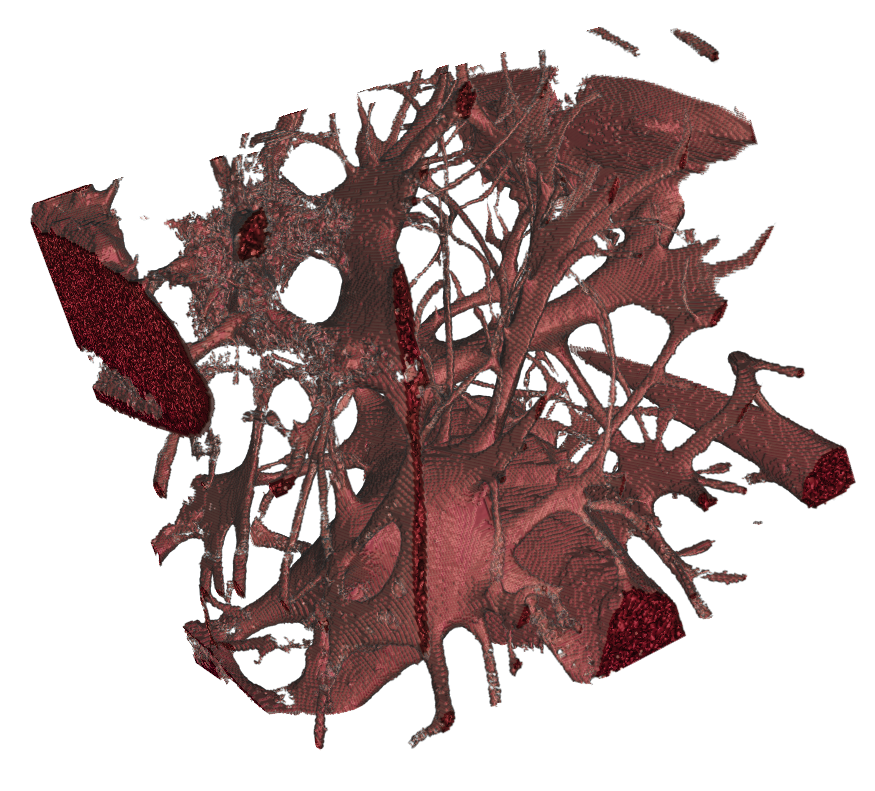
\includegraphics[width=\linewidth,height=\linewidth]{figures/blood_new_cube.png}
        \caption{3D render of a $1mm \times 1 mm \times 1 mm$ cube of the blood network in the new bone region.}
        \label{fig:blood-new-cube}
    \end{subfigure}
    \caption{3D renders of the blood network. All of the samples are generated from a 2x downsample of the full resolution. Note the difference between the the capillary network in the old bone region (\ref{fig:blood-old-slice},\ref{fig:blood-old-cube}) compared to the newly grown bone region (\ref{fig:blood-new-slice},\ref{fig:blood-new-cube}).}
    \label{fig:blood-network}
\end{figure}

\subsubsection{Sub-classification of soft tissue}

With a good separation of soft tissue and bone, we map out the blood vessel network using connected
components analysis, which is visualized in the 3D renders in~\Cref{fig:blood-network}.
Here we see that we have successfully segmented the blood vessels out of the bone region.
It is especially prominent when looking at the capillary network, as we can see these in fine detail.
Noteworthy, the newly formed bone region (\Cref{fig:blood-new-slice}) contains a larger concentrations of these small blood vessels, compared to the old bone (\Cref{fig:blood-old-slice}).
If we zoom in to a small cube region (\Cref{fig:blood-old-cube} and \Cref{fig:blood-new-cube}), we see it even more defined, clearly seeing how the larger vessels connect through the smaller ones.

The osteocytes are selected by volume and shape: For every connected component
in the feasible volume range, its principal axis and best ellipsoid is computed and checked against
the potential osteocyte shape.

\subsection{Assessing bone-implant contact and blood-implant contact}

\begin{figure}
  \centering
  \begin{tabular}{c}
    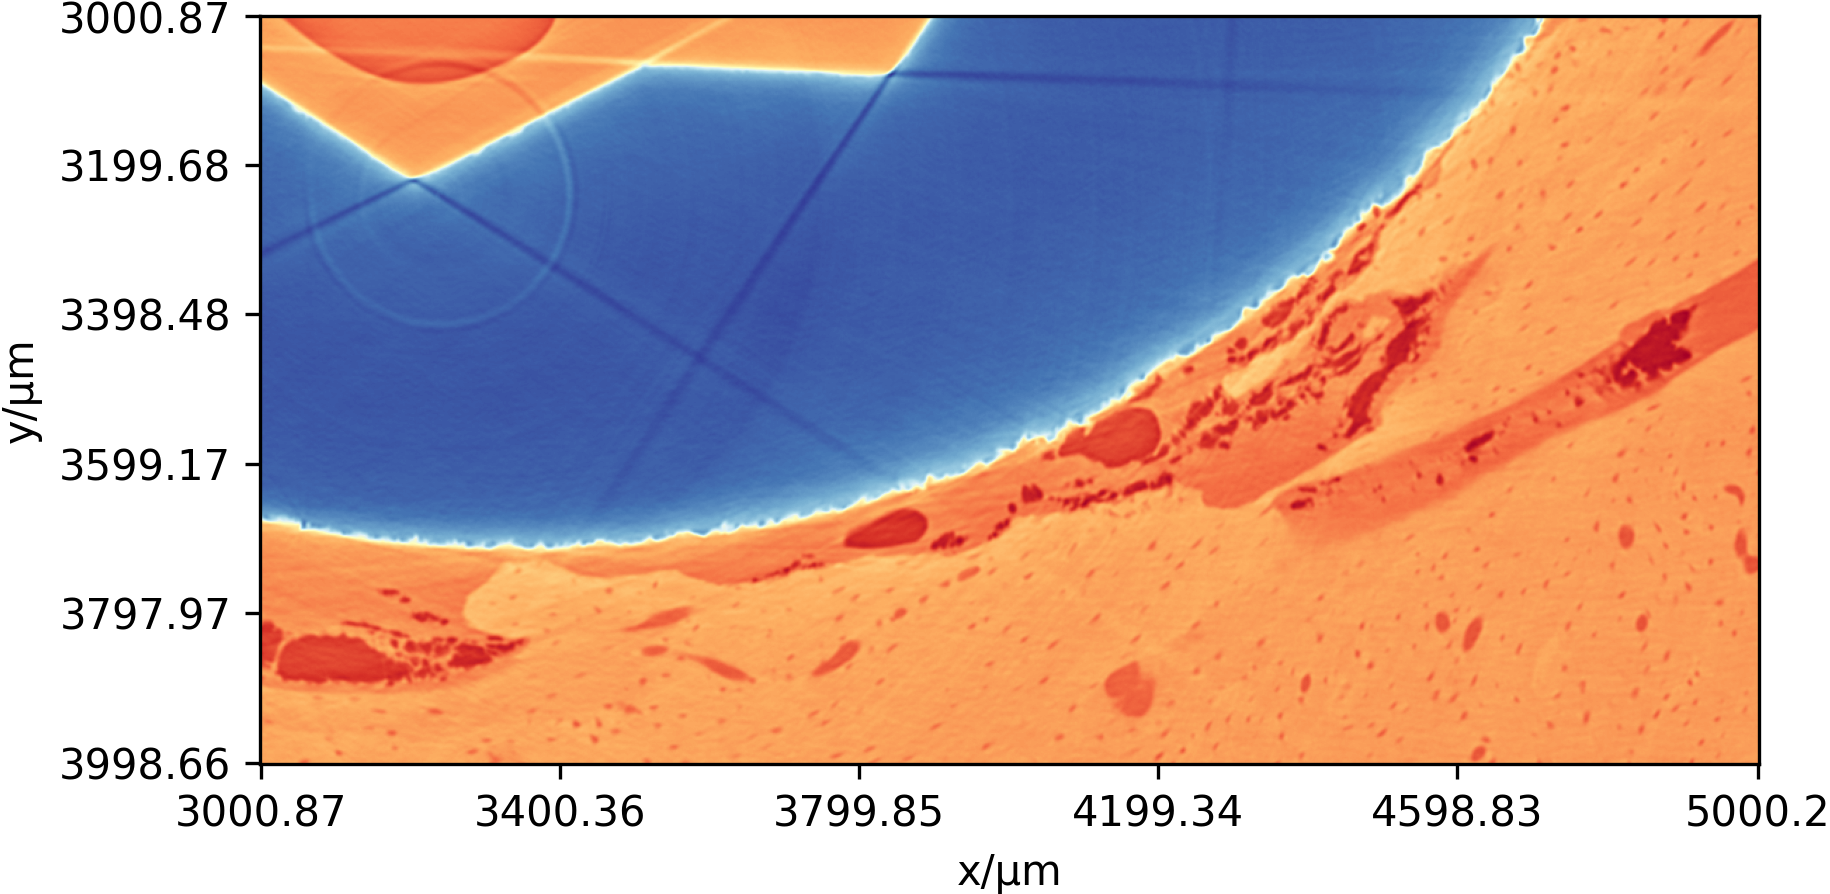
\includegraphics[width=\linewidth]{770c_pag-bic-xy-1x} \\
    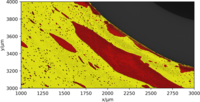
\includegraphics[width=\linewidth]{770c_pag-bic-P01-xy-1x}
  \end{tabular}
  \caption{XY slices of the original tomography (top), and the classified (bottom). The voxels are coloured according to the modeled probability functions $P(m|x,\fval)$ between 0 and 1: completely red voxels have $P(0|v,\fval) = 1$, completely yellow voxels have $P(1|v,\fval) = 1$, and uncertain voxels become progressively gray.
  }
  \label{fig:histology-comparison1}
\end{figure}

\begin{figure}
  \centering
  \begin{tabular}{c}
    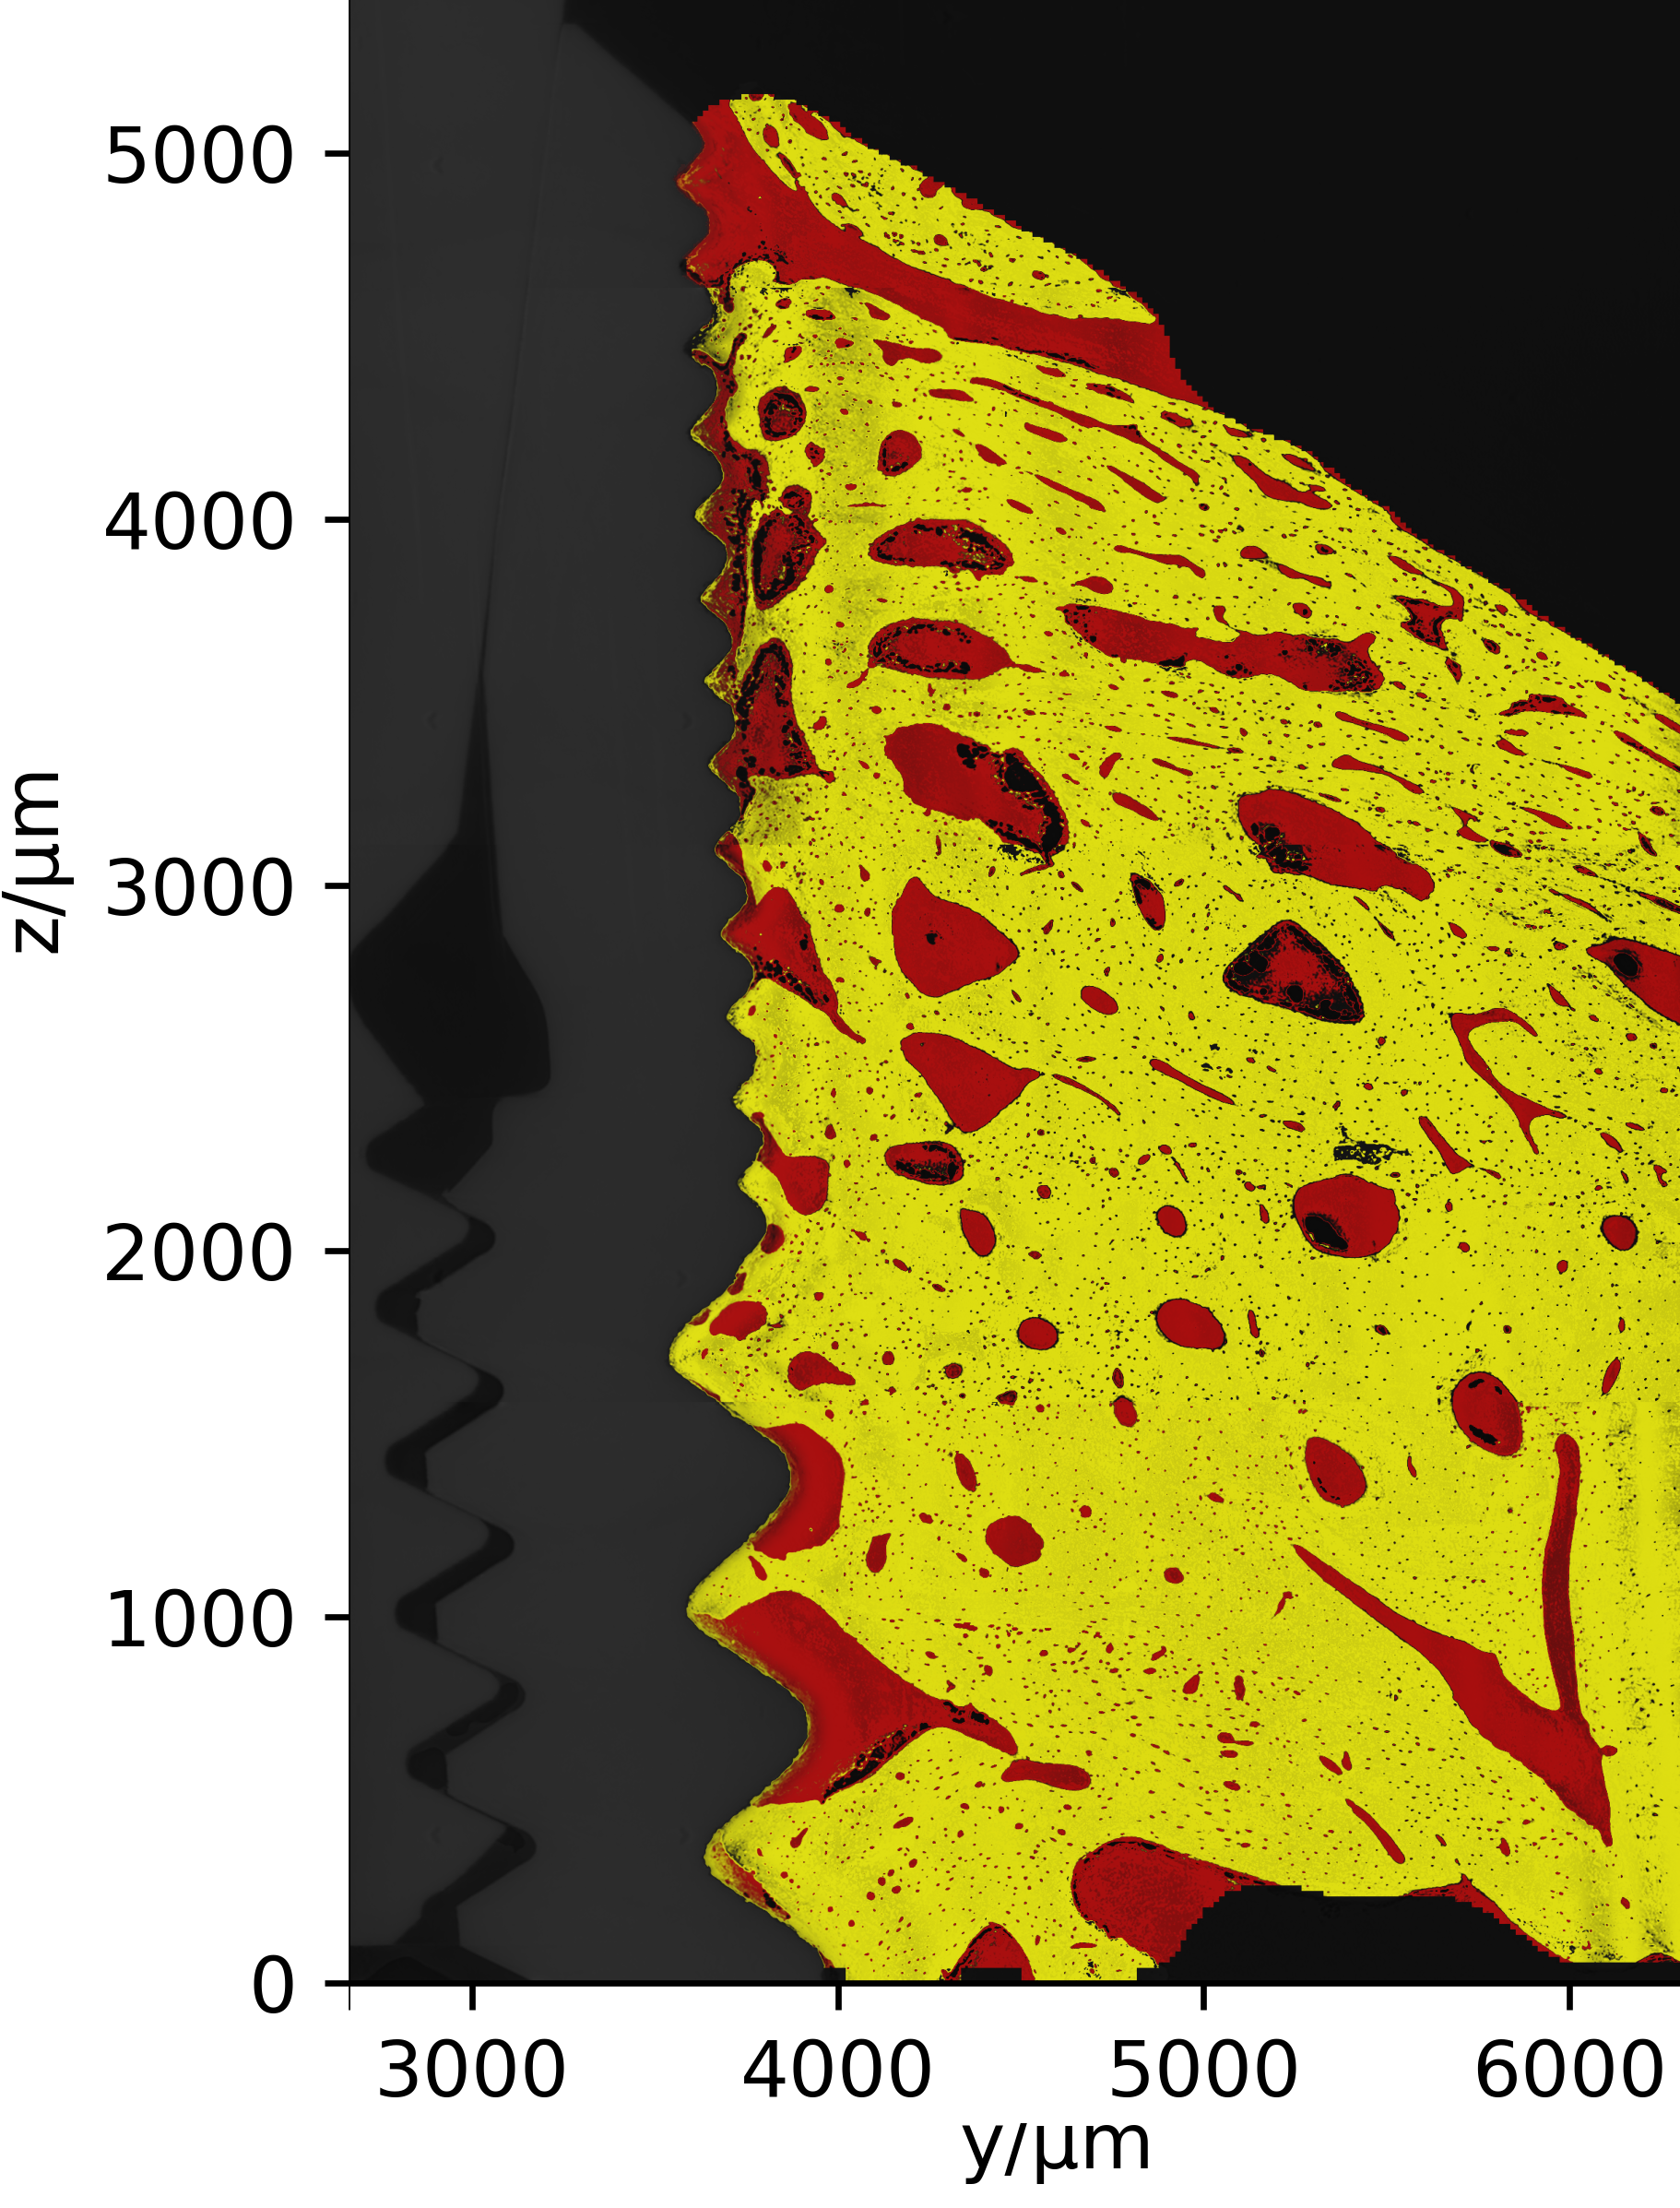
\includegraphics[width=.9\linewidth]{770c_pag-full-P01-yz-1x-gimp} \\
    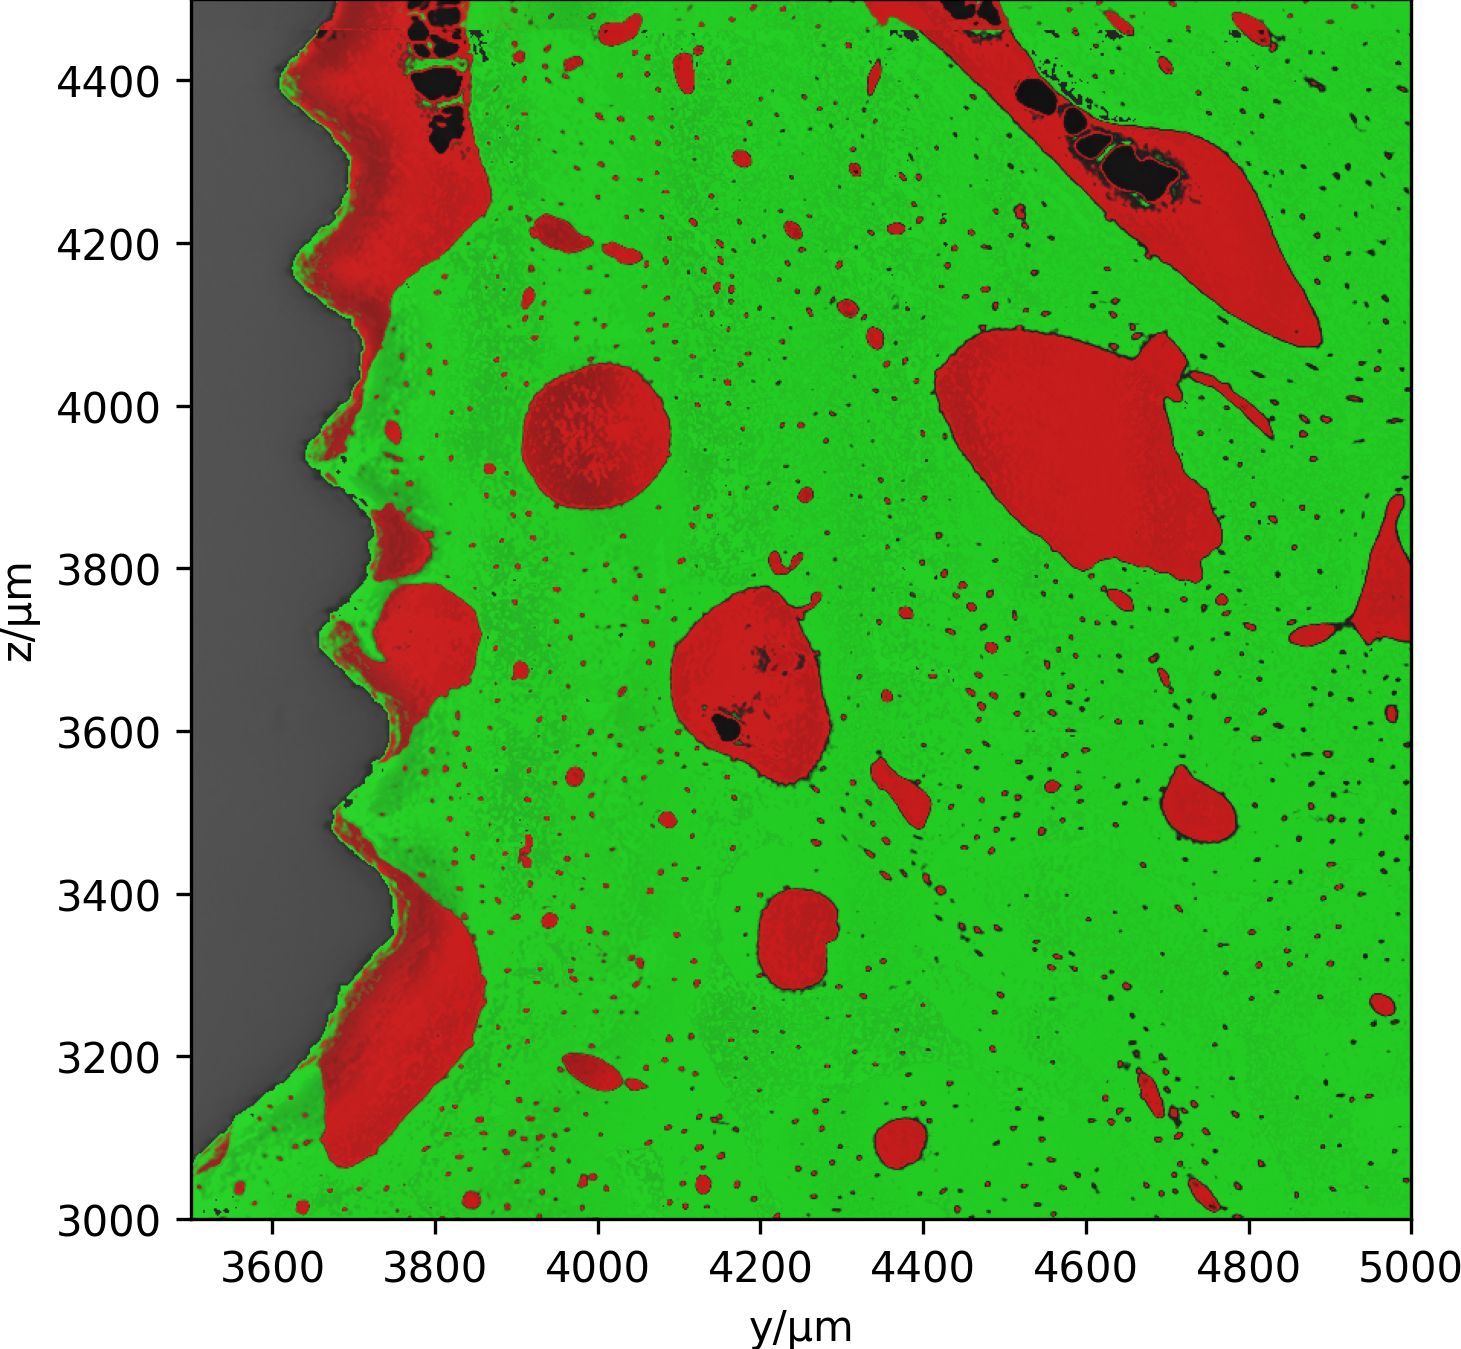
\includegraphics[width=\linewidth]{770c_pag-bic-P01-yz-1x}
  \end{tabular}
  \caption{ZY slices of the segmentation seen far away (top) and zoomed in (bottom). Yellow depicts bone and red depicts soft-tissue. Note that the segmentation correctly classifies the materials close to the implant, even in the grooves of the screw threads..}
  \label{fig:histology-comparison2}
\end{figure}


Once segmented, tissue in contact with the implant can be studied using the
Euclidean Distance Transform (EDT) from the implant, restricted to the bone region. We can
simply mask the voxels that are within a thin shell of distances, $d_{min} < d(x,y,z) \le d_{max}$,
for example $d_{min} = 1\mu m$ to $d_{max} = 5\mu m$. We then sum over the masked voxels of each
tissue type to obtain and divide by the total to obtain the tissue-to-implant contact per area,
or study the distribution across the surface area qualitatively.

A larger quantitative study is planned that analyses the full data set against recently conducted 
histological microscopy taken from the same biopsies. In the present work, we evaluate qualitatively:
Since the SR$\mu$CT tomograms are
clear enough that it is possible as humans to distinguish between blood vessels and bone,
as our mammalian visual cortex automatically corrects for the distortion effects, we can verify
the success of the automatic classification.

Figures \ref{fig:histology-comparison1} and \ref{fig:histology-comparison2} show the same 2D slices
as were shown in Figures \ref{fig:3viewsample} and \ref{fig:slices}, allowing us to visually inspect
them side by side. The voxels are coloured according to the segmentation confidence, with
degree of red proportional to the modeled probability $P(0|v,\fval)$ and degree of yellow proportional
to $P(1|v,\fval)$. Grey voxels indicate low model probabilities of both: either due to the voxel belonging
to another material, or simply low computed confidence of the model.
By comparing against Figures \ref{fig:histology-comparison1} and \ref{fig:histology-comparison2},
we see that the computed classification matches the human classification everywhere where it
is possible to visually distinguish the voxels. However, in a thin 1-voxel border
to the implant, we cannot verify the segmentation, as the voxel values are so blended together
with the implant voxel values that they become indistinguishable. A further strengthening of the analysis
is needed in order to reach this layer. It is possible that the information is irretrievably lost, or perhaps it
can be retrieved through a deconvolution - or simply a more precise version of the present analysis.


% \subsubsection{Cylindrical projection of implant contact-surface}

% In this subsection, we show how to map the tissue-to-implant contact surface for visual inspection.
% The challenge is that the equidistant region forms a curved surface that cannot simply be flattened.
% Instead, we project the voxels onto a cylinder, as shown in Figure \ref{fig:cylinder1}.

% \begin{figure}
%   \centering
%   \begin{tabular}{cc}
%     (a) & \begin{tabular}{c}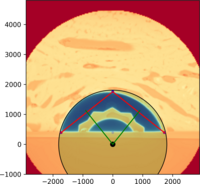
\includegraphics[width=.8\linewidth]{implant-FoR_prime-circle}\end{tabular} \\
%     (b) & \begin{tabular}{c}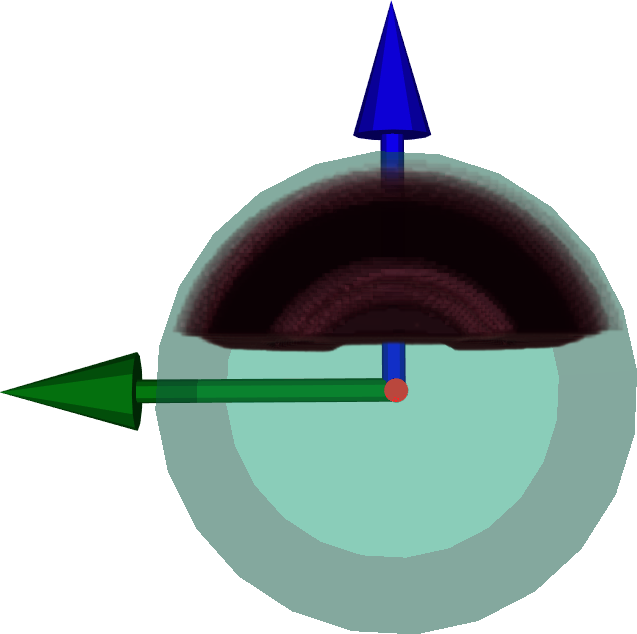
\includegraphics[width=0.4\linewidth]{implant-FoR_cylinder-y}%
%   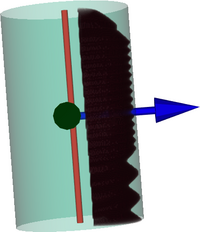
\includegraphics[width=0.5\linewidth]{implant-FoR_cylinder-z2}\end{tabular}
%   \end{tabular}
%   \caption{
%     (a) The implant is divided into 100 segments along its principal axis,
%     and for each segment, the circumscribed circle is computed.
%     (b) The best overall cylindrical fit for the implant is computed using
%     least squares. The implant contact is projected onto this cylinder,
%     and can now be shown in a flat plot.}
%   \label{fig:cylinder1}
% \end{figure}





%%% Local Variables:
%%% mode: latex
%%% TeX-master: "main"
%%% End:
